\documentclass[12pt]{report}

\usepackage[utf8]{inputenc}
\usepackage[french]{babel}
\usepackage[T1]{fontenc}
\usepackage{graphicx}
\usepackage{geometry}
\usepackage{hyperref}
\usepackage{amssymb}
\usepackage{amsmath}
\usepackage{amsfonts}
\usepackage{cite}
\usepackage[final]{pdfpages}
\usepackage{appendix}

\geometry{
    top=2.5cm,
    bottom=2.5cm,
    left=2.5cm,
    right=2.5cm
}

\bibliographystyle{plain}

\begin{document}

%----------------------------------------------------------------------------------------
%	TITLE PAGE
%----------------------------------------------------------------------------------------

\begin{titlepage} % Suppresses displaying the page number on the title page and the subsequent page counts as page 1
	\newcommand{\HRule}{\rule{\linewidth}{0.5mm}} % Defines a new command for horizontal lines, change thickness here
	
	\center % Centre everything on the page
	
	%------------------------------------------------
	%	Headings
	%------------------------------------------------
	
	\textsc{\LARGE Rapport de stage de fin d'étude d'école d'ingénieur.e}\\[1.5cm] % Main heading such as the name of your university/college
	
	\textsc{\Large Ecole Centrale de Marseille}\\[0.5cm] % Major heading such as course name
	
	\textsc{\large Laboratoire de Neurosciences Cognitives de Marseille}\\[0.5cm] % Minor heading such as course title
	
	%------------------------------------------------
	%	Title
	%------------------------------------------------
	
	\HRule\\[0.4cm]
	
	{\huge\bfseries Indexer la complexité linguistique en lien avec la dynamique cérébrale à partir de signaux MEG}\\[0.4cm] % Title of your document
	
	\HRule\\[1.5cm]
	
	%------------------------------------------------
	%	Author(s)
	%------------------------------------------------
	
	\begin{minipage}{0.4\textwidth}
		\begin{flushleft}
			\large
			\textit{Auteur}\\
			Lucas \textsc{Becquet} % Your name
		\end{flushleft}
	\end{minipage}
	~
	\begin{minipage}{0.4\textwidth}
		\begin{flushright}
			\large
			\textit{Tuteur et tutrice}\\
			Jean-Luc \textsc{Blanc} \newline
			Anne-Sophie \textsc{Dubarry}% Supervisor's name
		\end{flushright}
	\end{minipage}
	
	% If you don't want a supervisor, uncomment the two lines below and comment the code above
	%{\large\textit{Author}}\\
	%John \textsc{Smith} % Your name
	
	%------------------------------------------------
	%	Date
	%------------------------------------------------
	
	
	
	%------------------------------------------------
	%	Logo
	%------------------------------------------------
	
	\vfill\vfill
	
\includegraphics[width=0.6\textwidth]{logos.png}\\[1cm] % Include a department/university logo - this will require the graphicx package
	 
	%----------------------------------------------------------------------------------------
	\vfill\vfill\vfill % Position the date 3/4 down the remaining page
	
	{\large Avril-Septembre 2023} % Date, change the \today to a set date if you want to be precise
	
	\vfill % Push the date up 1/4 of the remaining page
	
\end{titlepage}

\chapter*{Résumé}

Dans ce rapport de stage de fin d'étude, on aborde la complexité des activités cognitives lors de la compréhension de phrases avec une démarche inter-disciplinaire des systèmes complexes en nous référant principalement aux formalismes de la théorie de l'information et des systèmes dynamiques \cite{8}. Dans ce contexte, on explore la compréhension linguistique sur la base de mesures de signaux neurophysiologiques, issus de l'activité cérébrale, collectés à partir d'un magnétoencéphalographe (MEG). Ces mesure permettre de capturer la dynamique cérébrale que l'on cherche à indexer à différentes conditions expérimentales, qui reflètent difféents degrés de complexité linguistique.

Sur le plan méthodologique, on a utilisé une approche basée sur la représentation symbolique d'un système dynamique. Ces méthodes permettent de quantifier la complexité intrinsèque de la dynamique cérébrale et la quantité d'information produite lors de la compréhension linguistique.

\chapter*{Remerciements}

J'aimerais remercier tout d'abord toute la communauté scientifique à laquelle j'appartiens, qui, depuis tout temps, s'évertue à dégager les concepts du monde puis à les définir, les représenter. Sans elle, mon travail n'existerait pas.

J'aimerais surtout remercier mon tuteur Jean-Luc Blanc et ma tutrice Anne-Sophie pour leur patience. Ils ont réussi à me transmettre leur passion pour les Neurosciences et la recherche, m'ont guidé et accompagné durant tout mon stage et se sont montré.e.s compréhensif et compréhensive, même dans les moments difficiles. 

J'aimerais également remercier Loïc Bonnier de l'équipe DI²S²C qui a toujours été là pour m'aider sur les aspects techniques de codage et avec qui l'ambiance était toujours stimulante et chaleureuse. J'aimerais aussi remercier Laurent Pezard qui m'a aidé et inspiré dans mes travaux et avec qui travailler était un plaisir.

Enfin, j'aimerais remercier mon père et ma mère, qui, depuis toujours, sont d'un soutien et d'une volonté de me comprendre sans égal.


\tableofcontents

\chapter*{Introduction}
\addcontentsline{toc}{chapter}{Introduction}
\section{Contexte}

J'ai eu la chance d'effectuer mon stage au Laboratoire de Neurosciences-Cognitives de Marseille (LNC). Ce laboratoire constitue un centre de recherche de pointe dans les domaines des Neuroscience et de la Psychologie cognitive avec le Laboratoire de Psychologie Cognitive de Marseille (LPC). Ces deux laboratoires fusionneront pour former le CRPN, à partir de janvier 2024.

\vspace{2ex}
J'ai travaillé au sein de l'équipe de Développement Informatique et Infrastructure Système pour les Sciences du Cerveau (DI²S²C). Cette équipe de soutien à la recherche a deux missions principales. Tout d'abord, certaines membres s'occupent de la La gestion, l'administration et la maintenance de l’infrastructure informatique du centre de recherche. La deuxième mission consiste en la participation à des projets de recherche en apportant notamment une expertise en informatique scientifique (développement d'applications, conseils méthodologiques, calcul scientifique etc ...). L'équipe DI²S²C est dirigée par Jean-Luc Blanc, ingénieur de recherche CNRS, qui m'a acceuilli et guidé avec Anne-Sophie Dubarry, ingénieure de recherche CNRS dans la même équipe, pendant ces 6 mois. La structuration de cette équipe est détaillée par un organigramme en Figure \ref{fig0.1}. J'ai également eu l'opportunité d'échanger avec François-Xavier Alario, directeur de recherche CNRS au LPC, sur les aspects psyco-linguistiques que comprend mon travail, notamment dans les choix à effectuer pour la segmentation temporelle du signal et l'interprétation des résultats. J'ai aussi pu avoir le plaisir de travailler avec Laurent Pezard, professeur dans l'équipe Dynamique Auditive Neuronale (DNA) au LNC, et qui m'a beaucoup apporté en termes de compétence de développement informatique et de démarche scientifique.

\begin{figure}[!ht]
    \centering
    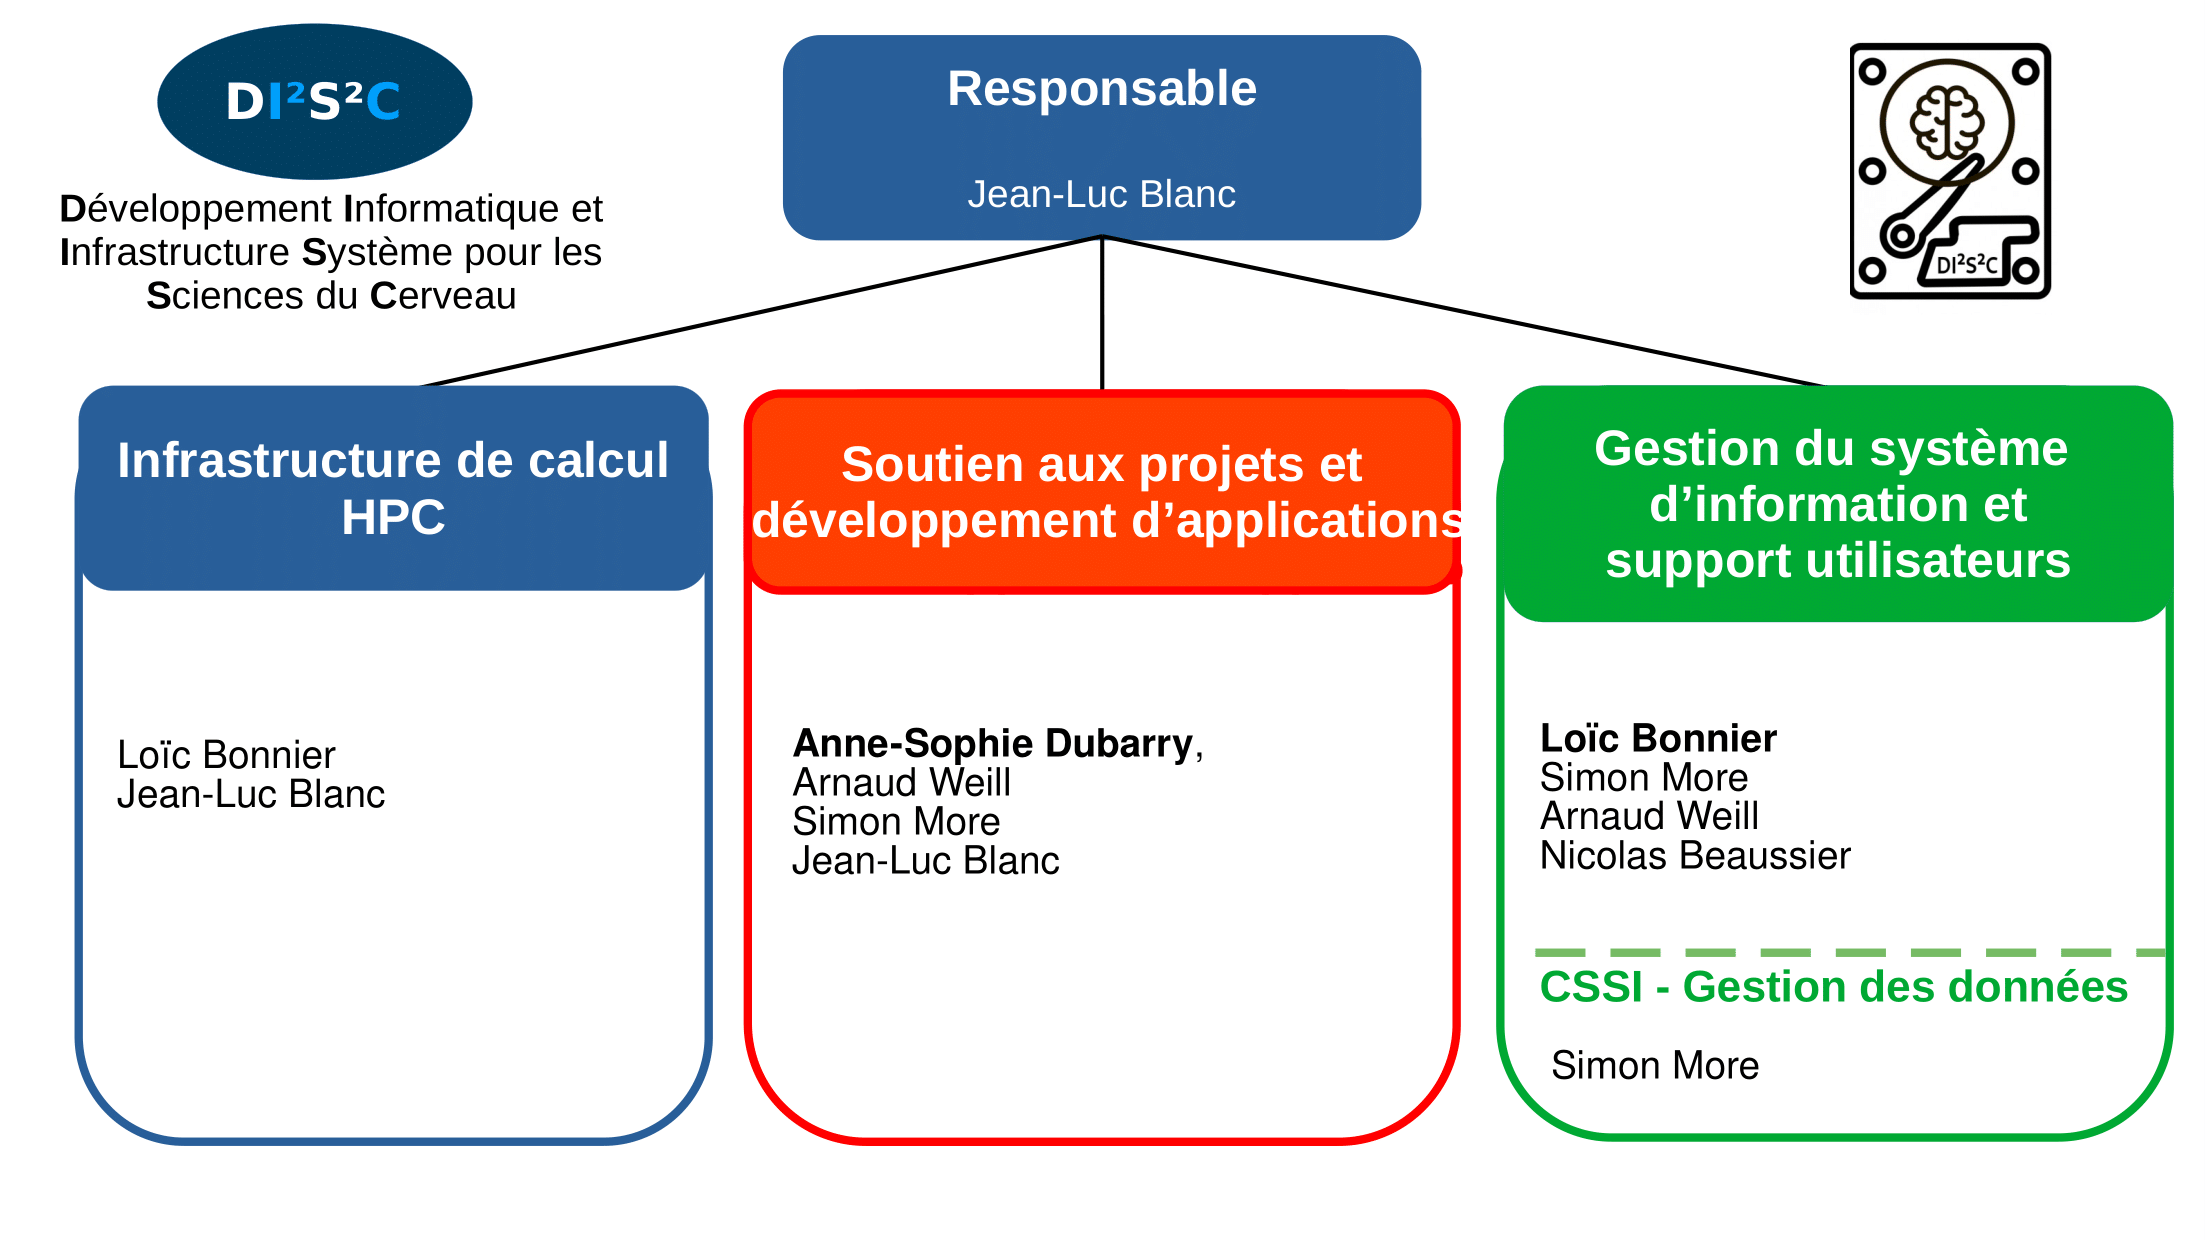
\includegraphics[width=13cm]{OrganigrameDISC.png}
    \caption{Organigrame de l'équipe DISC}
    \label{fig0.1}
\end{figure} 

\section{Objectifs du stage}

Durant ce stage, nous avions pour ambition de faire le lien entre complexité linguistique et la dynamique cérébrale. Que se passe-t-il dans le cerveau, en termes d'activation de population de neurones, lorsqu'une personne comprend, ou non, une phrase qu'elle lit ou qu'elle entend ?
La compréhension linguistique, qu’elle soit orale ou écrite, passe par la capacité à combiner des mots d’une phrase pour en saisir le sens; Qui a fait quoi ? A qui ? Ce n’est pas une simple concaténation. On s’intéresse donc à la dynamique cérébrale, au processus d’opérations cognitives qui permet la compréhension de chaque mot et de leur sémantique ainsi que la syntaxe et le contexte dans lesquels ils sont inscrits pour comprendre le sens de la phrase. 

Le point de départ de mon travail repose sur des enregistrements des champs magnétiques émis par le cerveau de par son activité (signal magnétoencéphalographique ou MEG). Ces données constituent une mesure de la dynamique cérébrale que j'ai étudié. L'objectif de mon stage était donc de mettre en place un algorithme permettant d'extraire des représentations symboliques à partir de segments des séries temporelles du signal MEG (Figure \ref{fig0.2}), découpées en fonction des différents stimuli. Ces stimulis correspondent à différents degrés de complexité linguistique. Par exemple, on peut s'intéresser à comparer l'activité cérébrale lors de la lecture ou de l'écoute de phrases simples par rapport à celle lors de phrases complexes au sens grammatical. On se focalisera sur la dynamique cérébrale liée à la compréhension de chaque mot d'une phrase. Ces représentations symboliques permettent de représenter un système dynamique continu (le cerveau) comme une séquence de symboles correspondants à des états discrets du système étudié. En effet, on se base sur l'espace des phases (ou espace des états) \cite{18} qui constitue l'espace mathématique dans lequel tous les états possibles du système sont représentés ; chaque état possible correspond à un point unique dans l'espace des phases. Cet espace permet de nous affranchir du temps en représentant les capteurs les uns en fonction des autres dans un hyperespace, où chacun d'eux représente un degré de liberté du système dynamique étudié. La représentation symbolique est une méthode qui permet d'associer un symbole à chaque partie de l'espace des phases en regard d'une partition comme illustré en (c) de la Figure \ref{0.2}. On a alors des séquences de symboles que l'on appelle séquences symboliques qui rendent compte de la dynamique cérébrale. En effet, chaque symbole correspond alors à un ou plusieurs états possibles (en fontion de la finesse de la partition) du système dynamique étudié. Cela permet de rendre compte de la complexité intrinsèque de la dynamique cérébrale et de la quantité d'information contenue dans celle-ci grâce à une métrique puissante : l'entropie.

\begin{figure}[!ht]
    \centering
    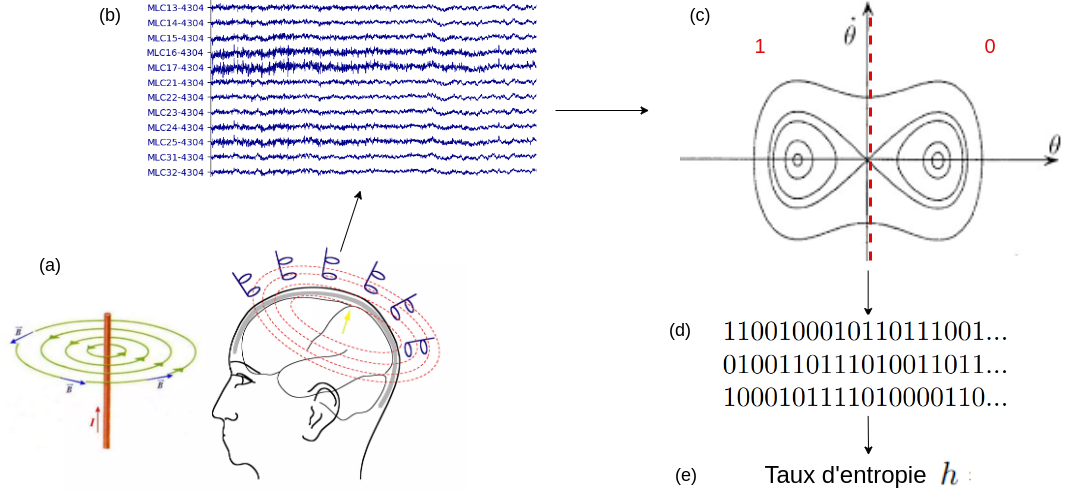
\includegraphics[width=17cm]{schema_algorithme.png}
    \caption{Schéma de l'algorithme mis en place durant le stage. (a) Mesure des champs magnétiques générés de par l'activité cérébrale. (b) Séries temporelles des capteurs. (c) Représentation symbolique de l'espace des phases des capteurs avec à une partition. Ici représenté en seulement 2 dimenions avec une partition binaire, les points des trajectoires à gauche de la ligne en pointillé rouge sont associées au symbole 1 tandis que ceux à droite au symbole 0. (d) Séquences symboliques représentées pour chaque capteur. (e) Taux d'entropie de chaque séquence symbolique.}
    \label{fig0.2}
\end{figure}

Le but est donc de calculer l'entropie de représentations symboliques associées à des conditions expérimentales et de les comparer entre elles. De cette manière, on lie la complexité linguistique et sa compréhension à la dynamique cérébrale associée. Cette métrique qu'est l'entropie est définie à l'intersection de 3 domaines. Dans le cadre de la théorie de l'information, l'entropie mesure la quantité d'information du signal d'origine qui a été produite par une source. Dans le cadre de la théorie des systèmes dynamiques, cette quantité rend compte de la complexité intrinsèque du système dynamique étudié en lien avec les notions d'ordre et de désordre. Enfin, dans le cadre de l'informatique théorique, l'entropie indique de la complexité du codage de la séquence symbolique permettant de décrire un phénomène observé par rapport à un alphabet universel. L'entropie est donc un indicateur, une métrique, qui nous renseigne sur la dynamique du système complexe que l'on étudie : le cerveau. Dans le cadre de cette étude, l'entropie nous permet donc mesurer l'effet de la complexité linguistique sur l'activité neuronale et de rendre compte de la dynamique cérébrale sous-jacente associée à la compréhension. 

La problématique de mon stage est donc la suivante : Peut-on discriminer des conditions expérimentales et rendre compte d'une compréhension linguistique sur la base de la quantification précise de la dynamique cérébrale ?

\vspace{2ex}
J'étudierai dans un premier temps l'origine neurophysiologique et les techniques d'enregistrement des signaux sur lesquelles nous travaillons avant d'introduire la base de données MEG que nous avons utilisée pour cette étude. J'expliquerai ensuite le processus de pré-traitement du signal MEG ainsi que la segmentation temporelle de celui-ci en regard des conditions expérimentales. Puis, je présenterai les concepts et les méthodes de la théorie de l'information et de la théorie des systèmes dynamiques que nous avons utilisé pour notre algorithme. Je me focaliserai principalement sur la représentation symbolique d'un système dynamique et l'entropie d'une séquence symbolique. Enfin, je détaillerai l'implémentation de l'algorithme mis en place au cours du stage et les résultats obtenus à partir des données expérimentales.


\chapter{Notions de neurophysiologie}

Nous avons décidé de travailler avec des données de magnétoencéphalographie comme mesure de l'activité cérébrale. Dans cette partie, nous allons alors expliquer comment sont générés ces signaux et comment en obtenir une mesure.

\section{De l'activité neuronale aux signaux neurophysiologiques}

Au sein de l'activité cérébrale, les neurones se transmettent des informations à l'aide de signaux électromagnétiques (au niveau des axones et des dendrites) et chimiques (au niveau des synapses). Les neurones corticaux sont regroupés en un réseau dense et constituent le cortex. Leur activation unitaire (c'est-à-dire le potentiel d'action) consiste en une dépolarisation transitoire de la membrane qui se propage le long des axones. Ces potentiels électriques, transmis le long des axones ou des dendrites, sont appelés courants primaires et correspondent à l'activation proprement dite des neurones \cite{5}. Lorsque ce courant se propage dans le milieu conducteur environnant (liquide céphalo-rachidien, crâne, peau, etc.), il devient un courant de volume. Ces deux types de courant s'additionnent dans le cortex et contribuent aux signaux neurophysiologiques. Lorsque les neurones sont orientés de façon aléatoire, les courants ont tendance à s'annuler. Parce qu'elles sont orientées orthogonalement à la surface de la substance blanche (c'est-à-dire à la surface du cortex), les cellules pyramidales, elles, contribuent principalement aux signaux enregistrés en neurophysiologie. Ces différents cas de figure sont illustrés en Figure \ref{fig1.1}.

\begin{figure}[!ht]
    \centering
    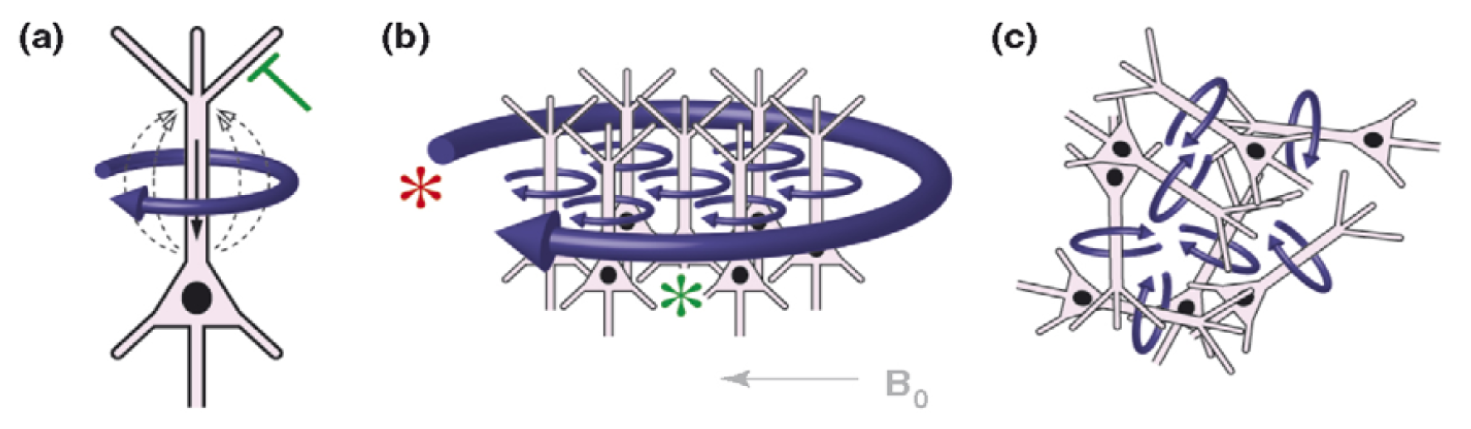
\includegraphics[width=12cm]{activation_neurones.png}
    \caption{Activation neuronale. (a) Neurone seul avec représentation de sont potentiel électrique (ligne pointillée) et du champ magnétique induit (flèche bleue). (b) Groupe de neurones orientés dans le même sens, leur activation synchrone crée un champ magnétique résultant. (c) Neurones orientés de manière aléatoire, les champs magnétiques s'annulent. Adapté de \cite{10}}
    \label{fig1.1}
\end{figure}

\vspace{2ex}
Lorsqu'un groupe de cellules neuronales contiguës s'active de manière synchrone, elles donnent naissance à un courant macroscopique. Lorsqu'il est détecté, il est représenté par un dipôle de courant. Comme la surface corticale est pliée, ces dipôles peuvent être orientés radialement ou tangentiellement par rapport à la surface du crâne.

\vspace{2ex}
La loi de Biot-Savard indique que pour un courant circulant le long d'un circuit en ligne droite, il existe un champ magnétique orienté de façon circulaire autour de cette ligne \cite{11}. Sa direction dépend de la direction de la charge électrique et est donnée par ce que l'on appelle la "règle de la main droite". Le pouce de la main droite pointe dans la direction du flux de courant (de la polarité négative à la polarité positive), les autres doigts pliés indiquent le sens du champ magnétique.

\vspace{2ex}
Cette propriété est importante car elle permet aux physiologistes et aux médecins d'explorer sous deux angles différents (avec des potentiels électriques et des champs magnétiques) la même activité cérébrale en recourant à des techniques différentes.

\vspace{2ex}
Cette activité reflète directement le traitement d'un ensemble de neurones spécifiques et peut être enregistrée de manière invasive (SEEG) ou non invasive (EEG, MEG).

\section{La technique d’enregistrement MEG}

L'activité cérébrale peut être mesurée à différentes échelles et à l'aide de différentes grandeurs. Il existe deux grandes familles de mesures de l'activité cérébrale : celles qui capturent les fluctuations hémodynamiques (modulations du flux, du volume sanguin, etc.), comme l'IRMf, et les mesures de l'activation neuronale réelle, comme l'EEG, la MEG et la SEEG (Figure \ref{fig1.2}). Ces dernières sont appelées techniques neurophysiologiques. Elles enregistrent l'activité électromagnétique des neurones, comme décrit dans la section précédente.

\begin{figure}[!ht]
    \centering
    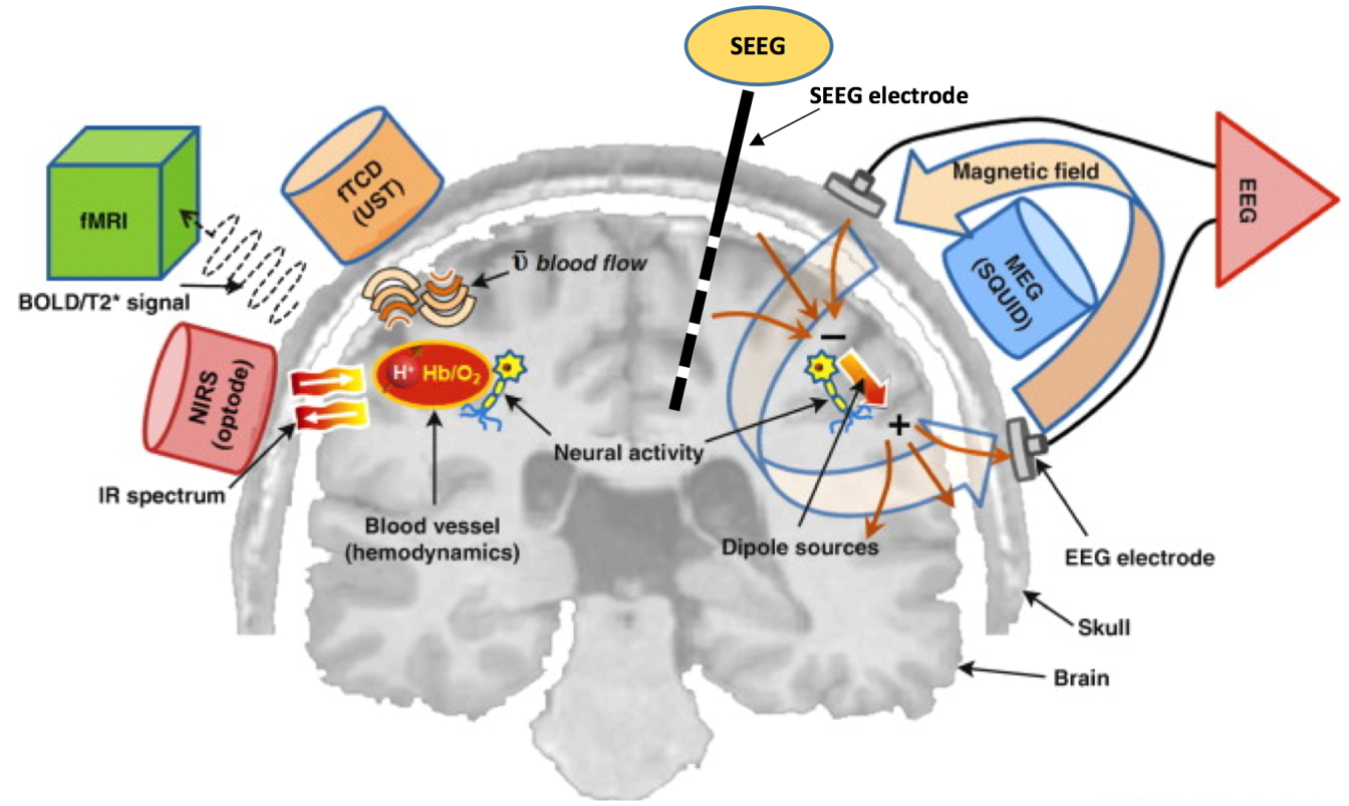
\includegraphics[width=12cm]{techniques_enregistrement.png}
    \caption{Illustration des différentes techniques d'enregistrement du cerveau. À gauche : techniques mesurant l'hémodynamique. À droite : Techniques neurophysiologiques. Adapté de \cite{12}}
    \label{fig1.2}
\end{figure}

\vspace{2ex}
L'EEG et la MEG sont les deux principales techniques d'enregistrement non invasives utilisées pour mesurer l'activité neurophysiologique au niveau du cortex entier. Il s'agit de techniques standards largement utilisées pour l'étude des activités physiologiques ou pathologiques dans les réseaux cérébraux à grande échelle, avec une résolution temporelle de l'ordre de la milliseconde \cite{9}. Elles se distinguent les unes des autres par la nature du signal recueilli. Alors que l'EEG mesure l'activité cérébrale en termes de potentiels électriques, la MEG enregistre les champs magnétiques provenant de l'activité cérébrale.

\vspace{2ex}
Il en va maintenant de se focaliser sur la technique d'enregistrement d'intérêt pour ce stage, à savoir, la MEG. Les paragraphes qui suivent présentent brievement son histoire ainsi que son fonctionnement.

\vspace{2ex}
Les premières mesures MEG ont été réalisées à la fin des années 1960 grâce à la collaboration de deux physiciens nord-américains : David Cohen et James Zimmerman. Initialement utilisés pour mesurer l'activité cardiaque, les premiers systèmes d'enregistrement MEG n'étaient composés que de quelques capteurs ; ce n'est qu'en 1992 que le premier système pour la tête entière a été construit. Aujourd'hui, les systèmes MEG disposent de plusieurs centaines de canaux organisés en forme de casque couvrant l'ensemble de la tête. Les champs magnétiques générés par l'activité cérébrale sont de l'ordre de quelques dizaines de femtoTesla ($10^{-15}$ Telsa jusqu'à des pico Telsa pour certaines activités cérébrales de grande amplitude telles qu'un pic épileptique). Ces champs très faibles peuvent être mesurés à l'aide de détecteurs magnétiques ultrasensibles appelés SQUID (superconducting quantum interference device), basés sur la supraconductivité et la physique quantique \cite{6}. Couplés à des bobines d'induction, ces dispositifs, immergés dans de l'hélium liquide, peuvent capter de très faibles fluctuations du champ magnétique provenant du cerveau comme on peut l'observer schématiquement en Figure \ref{fig1.3}. 

\begin{figure}[!ht]
    \centering
    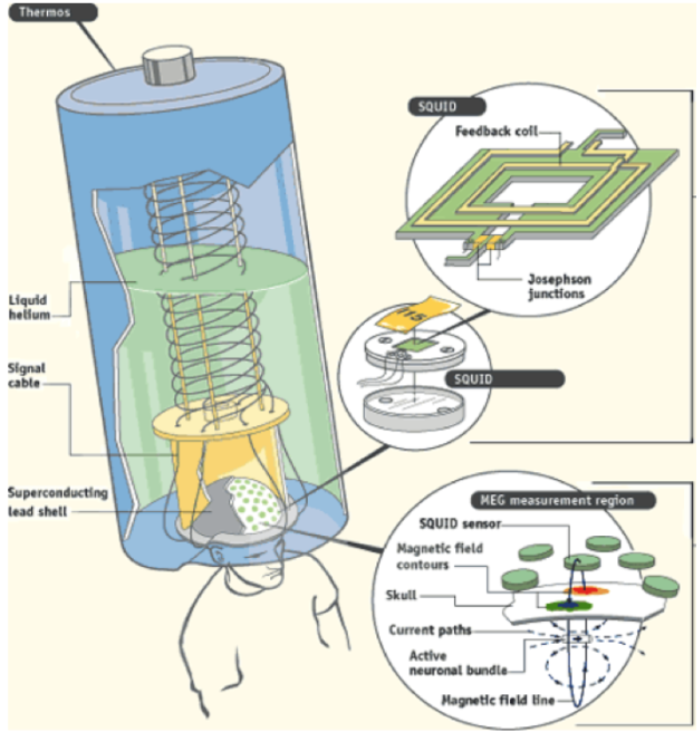
\includegraphics[width=15cm]{fonctionnement_meg.png}
    \caption{Illustration de la MEG. Schéma d'un système MEG complet et de ses composants (issu de \cite{5}).}
    \label{fig1.3}
\end{figure}

Comme ces champs magnétiques sont très faibles par rapport à tout autre champ magnétique (le champ magnétique terrestre qui est de l'ordre de $10^{-5}$ ou encore celui d'aimants qui peuvent aller jusqu'à quelques Tesla), un système MEG doit être installé dans une pièce à blindage magnétique pour permettre aux appareils de capter les faibles flucuations. Contrairement à l'EEG, il n'existe pas de position standard pour les capteurs (il n'y a qu'une seule taille de casque). Les positions des capteurs doivent être coregistrées en fonction de l'anatomie du sujet/patient. 

J'ai eu la chance de visiter le centre MEG de la Timone à Marseille, on pourra observer en Figure \ref{fig1.4} des photos prises des différents composants de leur système MEG.

\begin{figure}[!ht]
    \centering
    \includegraphics[width=15cm]{illustration_meg.png}
    \caption{Photographies des différents composants du système d'acquisition MEG, prises à différentes profondeurs. (a) Support pour le casque d'acquisition et aperçu de l'isolation du système. (b) Intérieur du dispositif une fois l'isolant retiré où l'on peut apercevoir les SQUID. (c) Gros plan sur les SQUID. (d) Plan correspondant à une prise de vue du dos de la photo précédente, on y voit les bobines.}
    \label{fig1.3}
\end{figure}


\chapter{Description du dataset (MOUS)}

On va dans cette partie présenter le jeu de données MEG sur lequel j'ai travaillé et expliciter les différents stimuli de compréhension linguistique auxquels les sujets ont été soumis. Cela nous permettra de nous approprier les données et de bien comprendre le protocole expérimental auquel les sujets ont été soummis. 
On souhaite appliquer notre algorithme à un dataset public d'étude de la compréhension linguistique, le Mother Of Unification Studies (MOUS) \cite{4}. 

L'étude a été réalisée sur un total 204 locuteurs natifs de Hollande et ayant comme langue maternelle le néerlandais. Il y a 100 hommes et 104 femmes, d'un âge moyen de 22 ans (de 18 à 33 ans). Dans la procédure de consentement éclairé, les sujets ont explicitement consenti à ce que les données anonymes collectées soient utilisées à des fins de recherche. Chaque sujet a effectué soit la tâche visuelle, soit celle auditive. Tous les sujets étaient droitiers, avaient une vision normale ou corrigée par le port de lunettes de vue. Ils n'avaient pas d'antécédents de déficits neurologiques, développementaux ou linguistiques. 

\vspace{2mm}
Ce dataset est structuré de la façon suivante : 
Il y a un total de 204 sujets répartis en deux moitiés pour deux tâches de compréhension linguistique différentes, une tâche visuelle et une tâche auditive. Pour chaque sujet, on dispose d'un enregistrement MEG d'une durée d'environ 1 heure.

\begin{figure}[!ht]
    \centering
    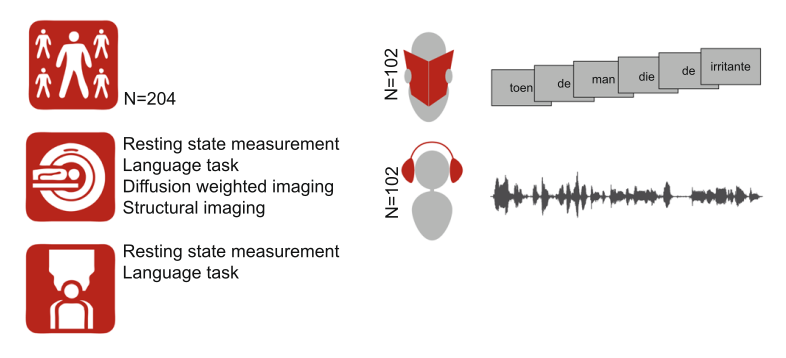
\includegraphics[width=10cm]{orga_dataset.png}
    \caption{Organisation du dataset. Issu de \cite{4}}
    \label{fig2.1}
\end{figure}

Les stimuli sont composés de 360 phrases en hollandais et leur analogues mélangés i.e une phrase ayant subi des permutations aléatoires entre les différents mots (donc inintelligibles a priori).

On a alors 
\begin{enumerate}
    \item 360 phrases, simples ou complexes (grammaticalement parlant)
    \item 360 listes aléatoires de mots 
\end{enumerate}

On rappelle qu'une phrase simple ne comporte qu'une seule proposition, donc un verbe conjugué. Tandis qu'une phrase complexe comporte plusieurs propositions, donc plusieurs verbes conjugués. Il y a donc naturellement plus de COD, COI et subordonnées au sein d'une phrase complexe.

\vspace{2ex}
Les phrases sont composées de 9 à 15 mots. Parmi ces différentes phrases, il y a :
\begin{enumerate}
    \item 180 phrases simples appelées simple relative clause sentence (RC-)
    \item 180 phrases complexes appelées relative clause sentence (RC+)
\end{enumerate}

\begin{figure}[!ht]
    \centering
    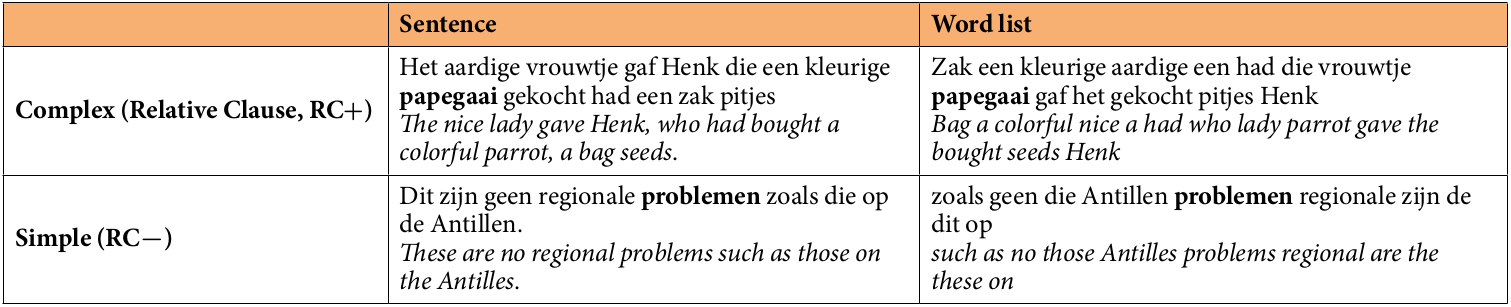
\includegraphics[width=20cm]{stimuli.png}
    \caption{Exemple des différents stimuli : Phrase simple (RC- sentence), phrase complexe (RC+ sentence) et listes aléatoires de mots associées. Issu de \cite{4}}
    \label{fig2.2}
\end{figure}

Chaque sujet est soumis à 180 phrases simples ou complexes donc à 180 sentences (RC+ ou RC-) ainsi qu’à 180 liste de mots aléatoires ou Random lists.

\vspace{2ex}
Sur chaque sujet, les phrases et les listes de mots aléatoires ont été utilisé le même nombre de fois.
Chaque phrase et sa liste de mots aléatoire associée contiennent un nom commun qui se trouve à la même position. Cette position peut varier de la 3ième à la 13ième position et ce mot est annoté comme cible ("target word").
Le mot placé en amont du "target word" ne diffère en taille d'un maximum de deux lettres entre la phrase et la liste de mots aléatoire associée.

\vspace{2ex}
Les stimuli sont soumis par blocs de 5 phrases ou 5 listes aléatoires de mots. Au début de chaque bloc, une présentation de 1500 ms indiquait le type de bloc : zinnen (phrases) ou woorden (mots). Dans les phrases, le premier mot commençait par une majuscule et le dernier mot se terminait par un point. 

\vspace{2ex}L'intervalle entre les essais a été réparti entre 3200 et 4200 ms. Pendant cette période, un écran vide était présenté, suivi d'une croix de fixation. C'est la phase d'instructions identifiée comme "Fixation picture, pre-trial baseline" et indexée par le nombre 20.

\begin{figure}[!ht]
    \centering
    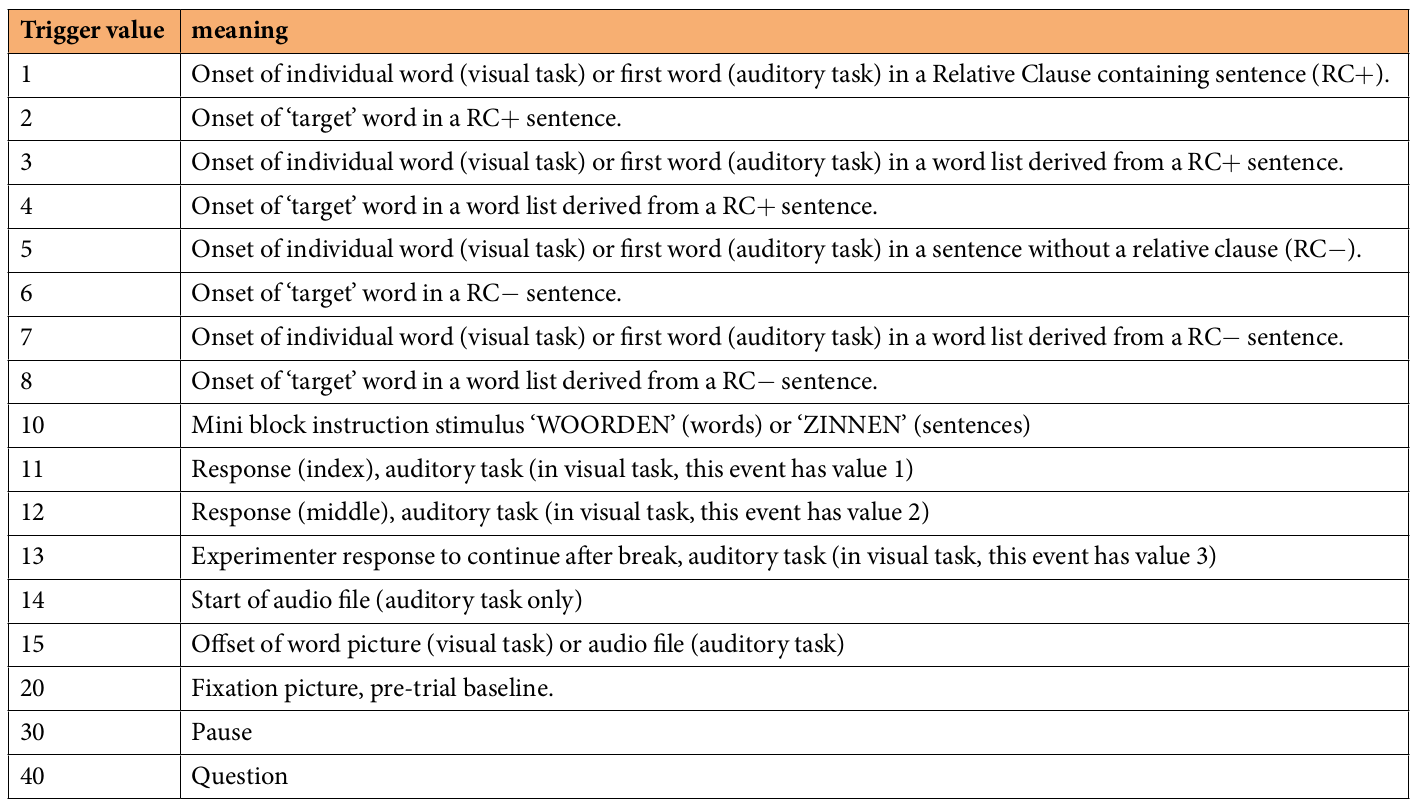
\includegraphics[width=20cm]{events_id.png}
    \caption{Identification des différents évènements et stimuli lors de l'enregistrement de la tâche de compréhension. Issu de \cite{4}}
    \label{fig2.3}
\end{figure}

Ce document va nous permettre d'identifier quels stimuli sont envoyés, un à un. Lors de l'analyse, cela permettra de segmenter les séries temporelles en courtes séquences appelées "époques" et donc de se focaliser sur les activités cérébrales d'intérêt par rapport à la tâche de compréhension linguistique.

\vspace{2ex}
On verra dans la partie suivante le pré-traitement que j'ai effectué sur les données ainsi que la manière dont j'ai segmenté le signal sur la base des différentes conditions expérimentales en se basant sur les événements.

\chapter{Pré-traitement des signaux MEG}

Avant de pouvoir appliquer l'algorithme développé durant le stage, il nous faut préparer les données.
Il existe différentes librairies et logiciels qui permettent le traitement de données MEG. Il me fallait une librairie développée sous le même language de programmation que celui que j'allais utiliser pour implémenter mon algorithme, de plus je bénéficiais du travail d'un ancien stagiaire, Hiroyoshi Yamasaki, qui avait réalisé un projet de recherche sur la compréhension linguistique avec MNE-Python. J'ai donc, sous les conseils de mes encadrants, choisi d'utiliser MNE-Python (\href{https://mne.tools/stable/index.html}{https://mne.tools/stable/index.html} \cite{17} qui est une librairie complète reconnue internationalement et développée sous Python. Cette librairie permet de manipuler des données MEG avec des fonctions de pré-traitement et d'analyse déjà implémentées. J'ai travaillé sous Linux et j'ai donc créé un environnement virtuel dans lequel j'ai téléchargé les modules et librairies Python dont j'avais besoin (MNE Python, numpy) afin d'avoir un environnement de codage stable et indépendant des mises à jour système. Cela me permet également de donner précisement l'état de mon environnement avec toutes les versions des librairies et toolbox utilisées pour que mon travail puisse être reproductible, suivant ainsi les bonnes pratiques scientifiques dans ce domaine \cite{13}.
Il existe trois grandes marques de systèmes d'acquisition MEG qui ont des caractéristiques différentes. Les enregistrements issus de ces différents systèmes se présentent sous le forme de structure de données de différents formats/types. Dans notre cas, l'enregistrement des données MEG a été réalisé avec une MEG de marque CTF. Ce système d'acquisition est essentiellement caractérisé par ses capteurs dits "gradiomètres axiaux". Un des avantages de MNE-Python est qu'il permet de simplement spécifier le type de système d'acquisition pour importer les données.

\vspace{2ex}
Les données MEG sont des données très complexes qui contiennent un certain nombre de meta-données permettant au Data analyst de retrouver le protocole d'enregristrement ainsi que les paramètres d'acquisition utilisés. En effet, on crée avec MNE-Python un objet que l'on appelle raw (pour brut, les données telles qu'elles ont été enregistrées) et qui contient les données MEG relatives à l'enregistrement d'un sujet. On manipule ensuite cet objet, on peut notamment afficher les meta-données relatifs à l'enregistrement (\ref{fig3.1}) avec la commande raw.info().

\vspace{2ex}
On prendra l'exemple d'un enregistrement de la tâche visuelle pour illustrer les propos.

\begin{figure}[!ht]
    \centering
    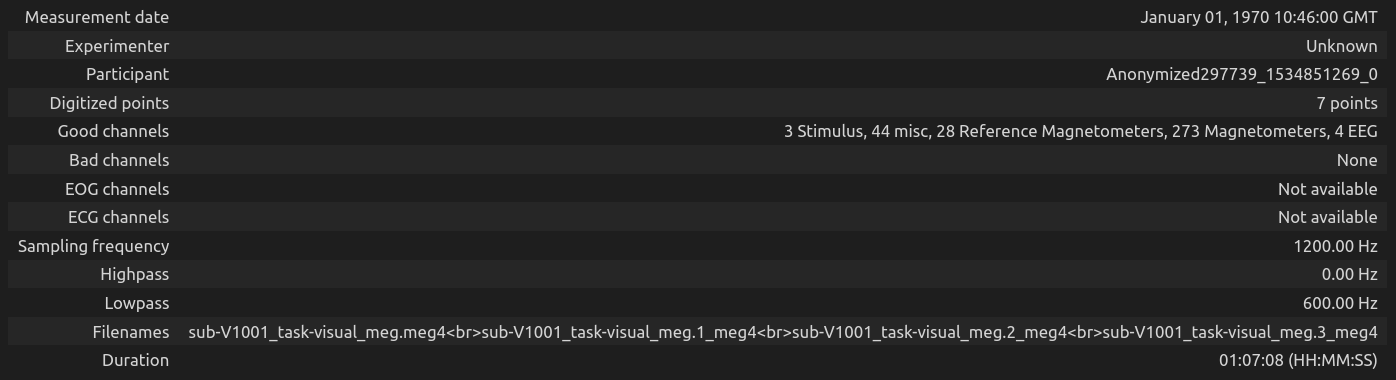
\includegraphics[width=16cm]{raw_info.png}
    \caption{Meta-données d'un enregistrement de la tâche de compréhension visuelle. On peut observer les différents canaux, y accéder aussi plus en détails, on voit aussi que la fréquence d'échantillonnage est de $1200 Hz$}
    \label{fig3.1}
\end{figure}
\section{Protocole de pré-traitement}

On présente ici (Figure \ref{fig3.2}) le protocole de pré-traitement des données qui a été mis en oeuvre durant le stage. 

\begin{figure}[!ht]
    \centering
    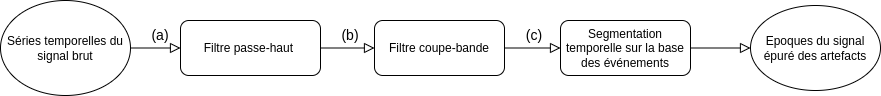
\includegraphics[width=15cm]{schema_pre_traitement.png}
    \caption{Protocole de pré-traitement des données MEG. (a) On applique d'abord un filtre passe-haut. (b) On applique un filtre coupe-bande. (c) On effectue la segmentation temporelle et donc la création d'époques des séries temporelles du signal MEG}
    \label{fig3.2}
\end{figure}

J'ai donc effectué les étapes de pré-traitement suivantes :

\begin{enumerate}
	\item Un filtre passe-haut avec une fréquence de coupure de $1 Hz$ afin de corriger la dérive lente ou "slow-drift" des séries temporelles;
	\item Un filtre coupe-bande autour de $50 Hz$ permettant de corriger le bruit des lignes éléctriques du signal MEG;
	\item Une ségmentation des séries temporelles en courtes époques en se basant sur les différentes conditions expérimentales afin d'appliquer l'algorithme mis en place durant le stage sur ces segments temporels d'intérêt.
\end{enumerate}

\section{Séries temporelles et filtre passe-haut}

Nous visualisons dans un premier temps le signal temporel pour repérer de potentiels artefacts visibles comme les battements du coeur ou les clignements des yeux.

Les artefacts limités à une plage de fréquences étroite peuvent parfois être réparés en filtrant les données. Les dérives lentes et le bruit des lignes électriques sont deux exemples d'artefacts limités à une plage de fréquences. Ce sont donc ces artefacts que nous avons traité afin de modifier le moins possible le signal d'origine et ainsi conserver de manière intacte la dynamique cérébrale.

\begin{figure}[!ht]
    \centering
    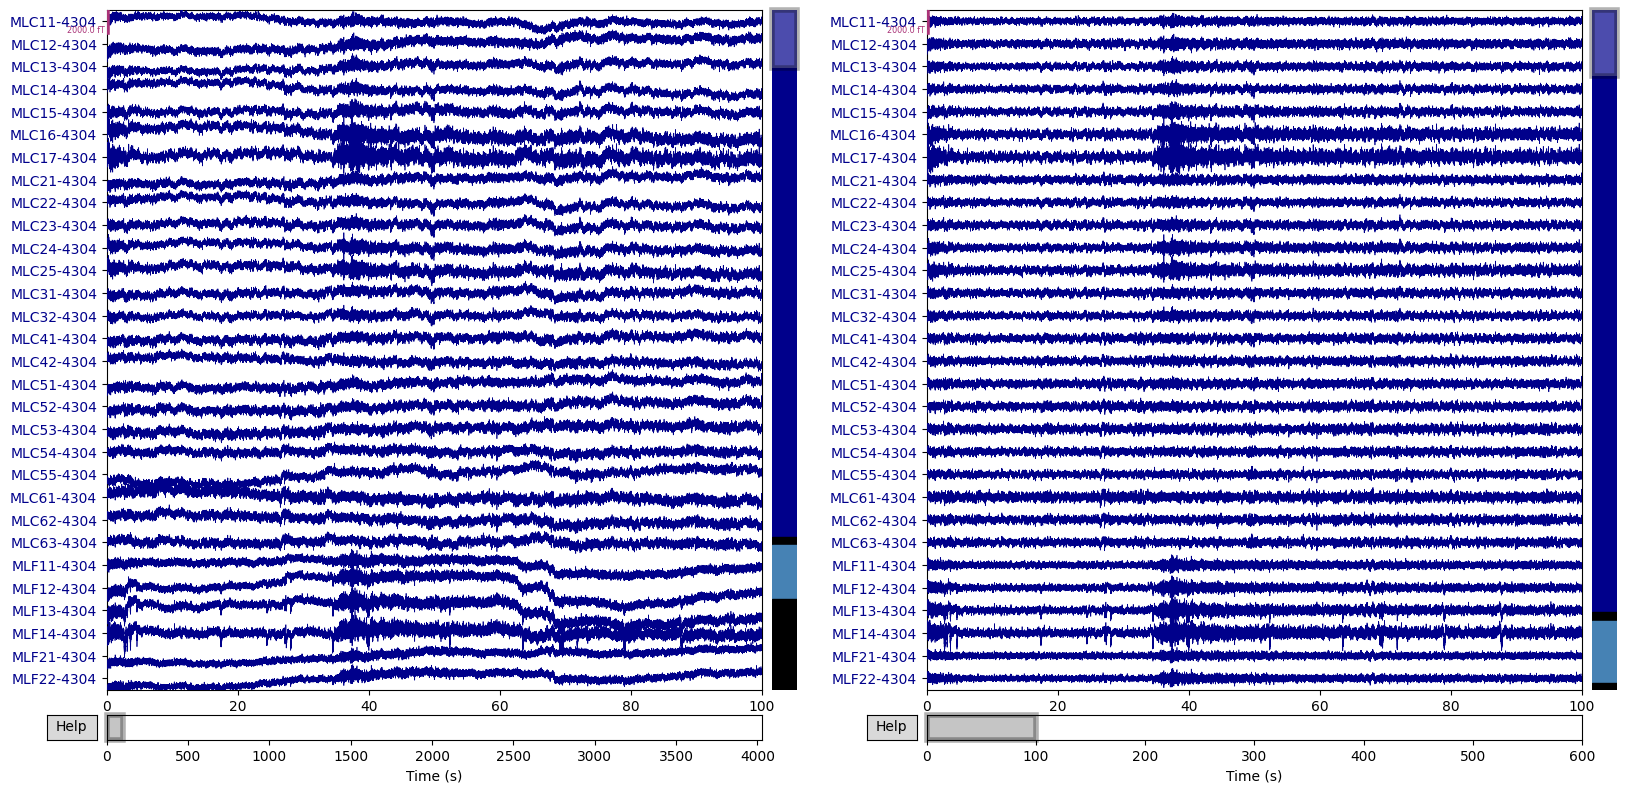
\includegraphics[width=13cm]{series_temporelles_effet_hp.png}
    \caption{A gauche, séries temporelles des différents canaux du signal MEG brut. A droite, séries temporelles après application du filtre passe-haut}
    \label{fig3.3}
\end{figure} 

On observe que les signaux ne sont pas centrés sur l'origine, ils dérivent. C'est là une dérive lente que l'on peut réparer en filtrant notre signal avec un filtre passe-haut avec une fréquence de coupure de $1 Hz$. 

\vspace{2ex}
Nous avons appliqué un filtre passe-haut pour corriger la dérive lente des séries temporelles. Par rapport, aux filtres coupe-bande, cela ne pose pas de problèmes car les activités fréquentielles du cerveau sont définies sur une plage de fréquence $\geq 1 Hz$. Après application du filtre passe-haut, le signal est à présent centré autour de 0.

\section{Spectre et filtre coupe-bande}

Il est essentiel de représenter les amplitudes en fonction des fréquences contenues dans le signal, comme en Figure \ref{fig3.4}. Ce type de représentation est appelé spectre; elle permet de mettre en évidence le contenu fréquentiel du signal.
On observe un pic à $50 Hz$ ainsi que ses harmoniques. Cette composante fréquentielle correspond au bruit dû à l'alimentation en courant du système d'acquisition, c'est le bruit des lignes électriques. Cet artefact environnemental se manifeste par des oscillations persistantes centrées autour de la fréquence de la ligne électrique, d'où le pic observé. 

\vspace{2ex}
J'ai donc utilisé un filtre coupe-bande à $50 Hz$ pour retirer la fondamentale du bruit des lignes éléctriques. J'ai fait le choix de ne pas appliquer de filtres coupe-bande pour retirer les harmoniques de cet artefact ($100 Hz, 150 Hz,...$) car même si la bande passante est très fine, cela risquerait de modifier significativement tout le signal et de perdre des informations quand à l'activité neuronale.

\begin{figure}[!ht]
    \centering
    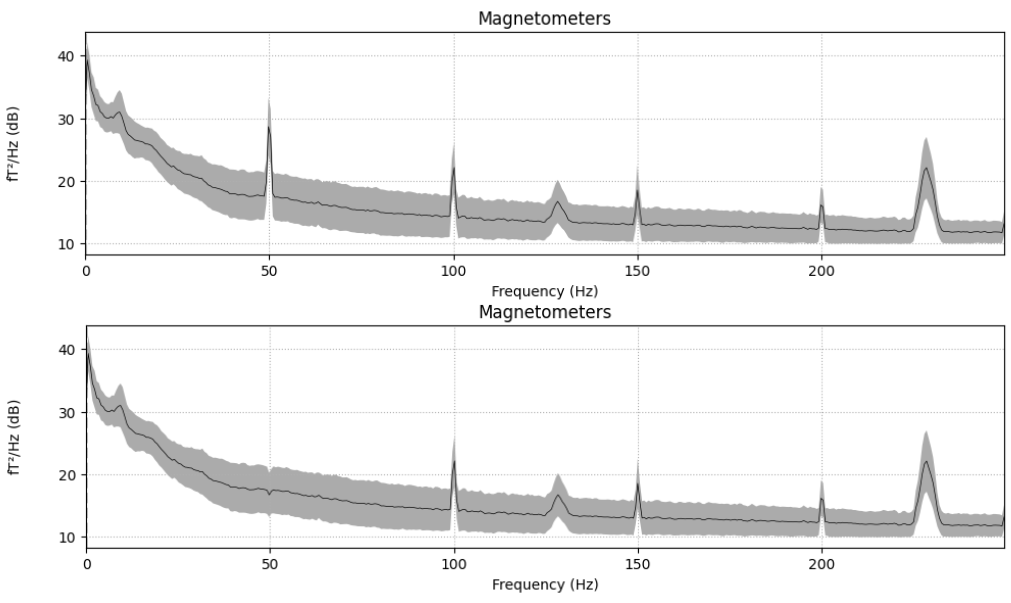
\includegraphics[width=13cm]{spectre_effet_coupe_bande.png}
    \caption{Graphe de la densité spectrale relatif à l'enregistrement d'un sujet de la tâche visuelle. En haut, le spectre du signal brut. En bas, le spectre du signal une fois le filtre coupe-bande à $50 Hz$ appliqué}
    \label{fig3.4}
\end{figure} 

\section{Segmentation temporelle du signal}

Une fois que les artefacts gênants pour l'étude ont été retirés des signaux MEG, il en va de le découper en courtes séquences que l'on appelle époques. En effet, pour réduire le rapport signal sur bruit, il faut appliquer l'algorithme développé au cours du stage sur une répétition de plusieurs segments temporels correspondants à un stimuli du même type (par exemple un mot cible d'une phrase simple), à une même condition expérimentale auquelle le sujet a été soumis. 

\vspace{2ex}
Les événements, dont on a présenté les différents types dans le chapitre précédent (Figure \ref{fig2.3}), sont une des méta-données de l'enregistrement MEG contenu dans le canal UPPT001 et nous renseigne sur la distribution des stimuli au cours du temps. Ces époques vont donc être selectionnées et découpées à partir des indexes temporels des différents événements (events). En effet, lors de l'enregistrement relatif à un sujet, il est renseigné une liste d'indexes temporels qui donne la trace du protocole expérimental. Cela permet de connaître le début d'une phrase et la caractérisation de celle-ci (simple, complexe, liste aléatoire de mots associée) et plus précisement l'apparition sur l'écran de chaque mot d'une phrase. 
Les événements sont cruciales pour l'analyse des données et un choix d'époques judicieux est indispensable pour obtenir des résultats significatifs. En effet, une fenêtre de temps trop grande, en prenant par exemple comme époque le signal MEG sur toute une phrase, a comme inconvénient de diluer l'activité cérébrale. Les premiers mots d'une phrase avant que la compréhension ne s'opère vont avoir une activité similaire à ceux d'une liste aléatoire de mots. Il est donc préférable de choisir une fenêtre de temps resserée autour de chaque mot pour définir les époques, en s'intéressant tout particulièrement aux target words.

\vspace{2ex}
On extrait les événements relatifs au protocole d'un sujet à partir du canal UPPT001 des données MEG. Cela nous permet de créer un objet event contenant les indexes temporels des différents événements. On renseigne ensuite un dictionnaire que l'on nomme event-id et dans lequel on fait correspondre les étiquettes (qui sont des entiers) des événements avec ce qu'ils signifient dans le protocole d'enregistrement (Figure \ref{fig2.3}). On peut visualiser en Figure \ref{fig3.5} le positionnement des événements dans le temps ainsi que le nombre de fois qu'ils apparaissent (sur 600 secondes d'enregistrement seulement, d'où l'absence de certains événements) :

\begin{figure}[!ht]
    \centering
    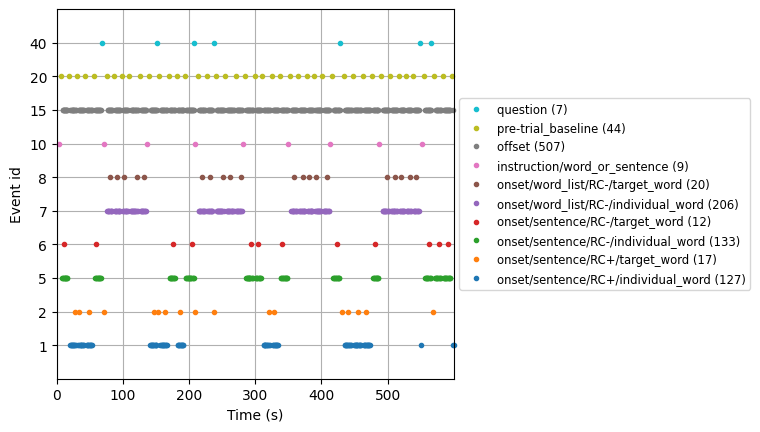
\includegraphics[width=17cm]{events_vis.png}
    \caption{Visualisation des différents événements au cours du temps d'un sujet de la tache visuelle}
    \label{fig3.5}
\end{figure} 

\vspace{2ex}
Par exemple, l'événement 5, "onset/sentence/RC+/individual-word" signifie l'affichage sur l'écran du sujet d'un mot individuel (qui n'est pas un target word) d'une phrase complexe. Sur la base de ces objets, on va créer des époques autour des événements d'intérêts.

\vspace{2ex}
Tout d'abord, on détermine l'écart maximum entre deux mots (et donc entre deux événements correspondants) d'une même phrase ou liste aléatoire de mots, cela nous permet de définir la durée que l'on choisira pour créer nos époques. Pour la tâche visuelle, on décide construire les époques en découpant le signal temporel sur chaque canaux 0.2 s avant l'affichage du mot et 1.2 s après. Ce qui nous fait des époques d'une durée de 1.4 s.

\vspace{2ex}
On discrimine ensuite les époques en fonction de l'événement d'intérêt. Dans notre cas, on construit des époques centrées autour des target words, d'autres autour des individual words, tout ça au sein des phrases simples et des listes de mots aléatoires issues de phrases simples. L'idée est de pouvoir comparer la dynamique cérébrale lors de la compréhension mot par mot entre la tâche visuelle et la tâche auditive, les phrases simples et leurs listes de mots aléatoires associées, les target words et les individual words.

\vspace{2ex}
Pour chaque époque, on a donc une matrice ayant pour lignes les 301 canaux et pour colonnes les valeurs que prennent les canaux sur le segment temporel que constitue l'époque, i.e., 1200 points.

\begin{figure}[!ht]
    \centering
    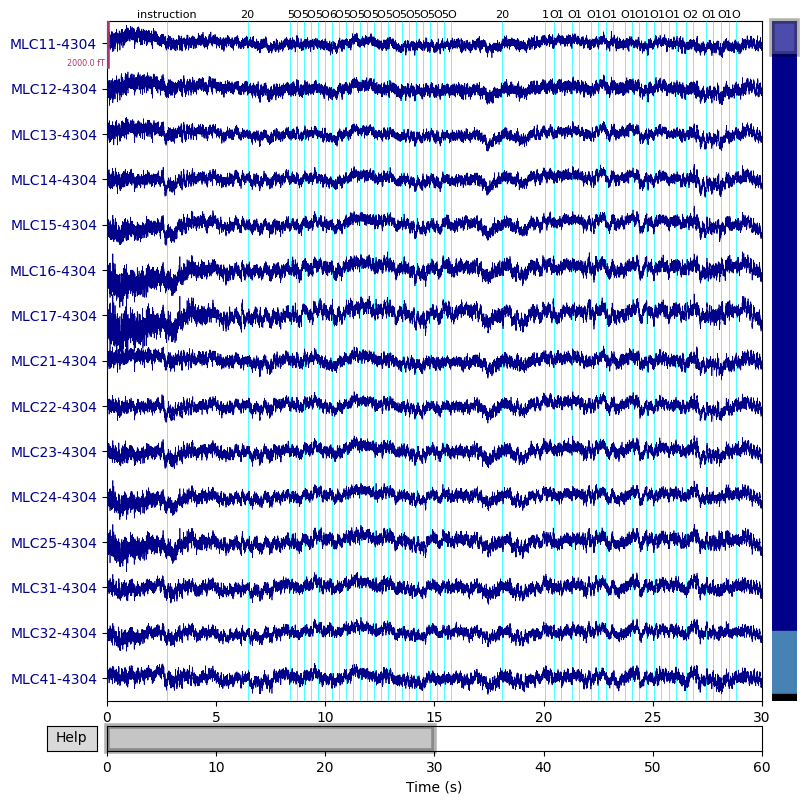
\includegraphics[width=13cm]{events_temporel.png}
    \caption{Visualisation des événements directement sur les différents canaux du signal temporel}
    \label{fig3.6}
\end{figure} 

\vspace{2ex}
Les données sont prêtes et nous avons créé les époques à partir des séries temporelles sur la base des différentes conditions expérimentales que nous souhaitons comparer. Nous pouvons à présent appliquer la partie centrale de l'algortihme mis en place durant le stage : la représentation symbolique de la dynamique cérébrale de conditions expérimentales et le calcul de l'entropie associée.

\chapter{Analyse dans le cadre de théorie de l'information}

Dans cette section, je vais introduire les fondements théoriques de l'approche de la théorie de l'information que j'ai utilisé. Plus particulèrement, la représentation symbolique et les indicateurs : l'entropie et le taux d'entropie d'une séquence symbolique.

\section{Représentation symbolique d'un système dynamique}

Je vais présenter le concept de représentation symbolique d'un système dynamique, i.e., comment extraire des séquences de symboles, qui rendent compte de la complexité du système dynamique d'intérêt, à partir de séries temporelles. Cela dans le but de calculer ensuite l'entropie associée à ce système.

\subsection{Théorie}

La méthodologie sur laquelle repose la démarche scientifique que nous avons choisi d'appliquer pendant mon stage est centrée autour du concept de représentation symbolique. En effet, on souhaite calculer l'entropie relative à différentes conditions expérimentales, i.e., un target word, un mot individuel, issu d'une phrase simple ou bien d'une phrase complexe, pour pouvoir ensuite les comparer entre elles. N'ayant pas accès de manière déterministe à la dynamique cérébrale mais ayant comme mesures de celle-ci les séries temporelles du signal MEG, il n'est pas possible de calculer directement l'entropie. En se basant sur la théorie des systèmes dynamiques \cite{3}, on va donc passer par un système dynamique discret isomorphe au système dynamique d'étude, c'est ce que l'on appelle la représentation symbolique. 

On définit dans un premier temps l'espace des phases (ou espace des états) \cite{18} qui constitue l'espace mathématique dans lequel tous les états possibles d'un système dynamique sont représentés ; chaque état possible correspond à un point unique dans l'espace des phases comme illustré en Figure \ref{fig4.1}. Cet espace permet de nous affranchir du temps en représentant les capteurs les uns en fonction des autres dans un hyperespace, où chacun d'eux représente un degré de liberté du système dynamique étudié, en l'occurence ici, la dynamique cérébrale.

La représentation symbolique peut être vue comme le fait de transformer les trajectoires dans l'espace des phases d'un système dynamique (séries temporelles) en une séquence d'états discrets représentés par un ensemble fini de symboles qui constitue les étiquettes des éléments de la partition. L'ensemble des symboles d'une séquence symbolique est appelé alphabet et correspond à la partition utilisée. Celui-ci est lié à la séquence symbolique et nous donne la trace de la représentation symbolique en question, i.e., la partition qui a été utilisée pour créer des représentations symboliques à partir des séries temporelles du système dynamique étudié.

\begin{figure}[!ht]
    \centering
    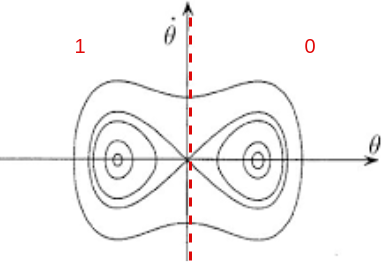
\includegraphics[width=8cm]{representation_symbolique.png}
    \caption{Illustration de la représentation symbolique dans l'espace des phases. Ici représenté en seulement 2 dimenions avec une partition binaire, les points des trajectoires à gauche de la ligne en pointillé rouge sont associés au symbole 1 tandis que ceux à droite sont associés au symbole 0.}
    \label{fig4.1}
\end{figure}

La dynamique symbolique revient donc à échanger des séries temporelles à valeurs continues d'un système dynamique contre des séquences symboliques avec un alphabet fini d'un système dynamique discret, qui sont les représentations symboliques. Les symboles de ces représentations sont les états discrets de la dynamique symbolique. Une séquence symbolique peut donc être vue comme un processus stochastique où la collection de variables aléatoires prend comme valeurs des symboles codés à partir d'un alphabet. En effet, une partition divise l'espace des phases en un nombre fini de régions. Chaque région se voit attribuer un symbole. Toute orbite de longueur infinie peut alors être convertie en une séquence symbolique en enregistrant la région de l'espace des phases que la trajectoire visite à chaque instant. Une représentation symbolique est donc une séquence de symboles qui rendent comptent des états discrets d'un système dynamique au cours du temps par rapport à une partition que l'on souhaite être génératrice dans l'espace des phases (espace des états).

L'entropie d'une séquence symbolique est une mesure qui nous donne énormément de renseignement. Dans le cadre de la théorie de l'information, l'entropie de Shannon nous renseigne sur la production d'information d'une source et l'imprévisibilité de celle-ci. Dans le cadre des systèmes dynamiques, l'entropie de Kolmogorov-Sinai $h_{\mu}(f) = sup h_{\mu}(f,\alpha)$ \cite{3} représente la quantité d'informations nécessaire pour reconstruire une trajectoire dans l'espace des phases à partir d'une condition initiale. Cela nous donne en fait la complexité de la dynamique intrinsèque du système observé et dans quelle mesure celui-ci est chaotique, i.e., désordonné. 

\vspace{2ex}
Le lecteur ou la lectrice trouvera les détails et les définitions mathématiques des concetps que l'on vient d'expliciter en annexe.

\subsection{Pratique}

La première manière de représenter symboliquement la trajectoire associée à notre système dynamique est d'extraire une séquence symbolique pour chaque série temporelle des canaux. Son principe est assez simple et on traite les canaux un par un. En effet, pour chaque canal, on mesure l'amplitude crête à crête du signal pour savoir dans quel intervalle le signal prend ses valeurs. On détermine alors l'histogramme des valeurs du canal en question que l'on va diviser par équipartition. En effet, à partir du nombre de symboles que l'on décide de fixer, i.e. la taille de l'alphabet, on découpe uniformément l'intervalle des valeurs en autant d'intervalles que l'on souhaite de symboles. On effectue ensuite l'attribution des symboles, i.e., les entiers qui sont étiquettes de chaque intervalles, aux points de la série temporel grâce à la fonction digitize du module numpy. 

\begin{figure}[!ht]
    \centering
    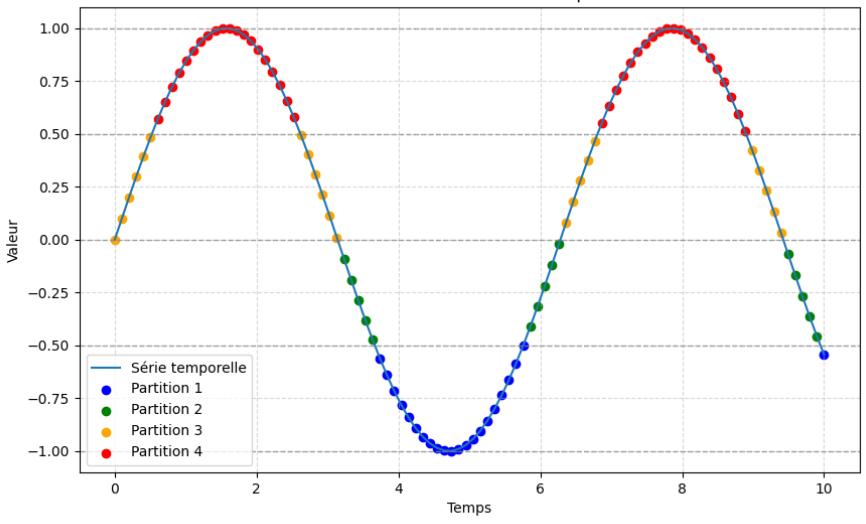
\includegraphics[width=13cm]{partition_serie_temporelle.png}
    \caption{Illustration d'une équipartition par histogramme des valeurs d'une série temporelle. Exemple d'une partition à 4 symboles d'une sinusoïde. On peut identifier les différents intervalles qui correspondent chacuns à un symbole de la partition}
    \label{fig4.2}
\end{figure}

En y associant un alphabet par défaut de la même taille que le nombre de symboles, on a alors une représentation symbolique de chaque canal et il suffit alors de créer les objets séquences symboliques correspondants grâce à la classe sequence du module scikits-symbolic que l'on présentera dans le chapitre suivant.

\vspace{2ex}
La deuxième façon d'effectuer une représentation symbolique de notre système dynamique que nous avons utilisé est une représentation symbolique dans l'espace des phases des capteurs. 
Pour se faire, on effectue une décomposition en valeurs singulières (SVD) \cite{20} de la matrice de nos données (capteurs $\times$ temps), plus précisement, comme la convention est d'avoir une matrice des données (temps $\times$ valeurs), on fait une décomposition en valeurs singulières de la transposée de notre matrice de données.

\vspace{2ex}
Soit $M$ la transposée de la matrice des données $m \times n$, la décomposition en valeurs singulières est définie par 

\begin{equation}
	M = USV^T
\end{equation}

\begin{enumerate}
	\item $U \in \mathcal{R}^{m \times n}$ contient un ensemble de vecteurs orhonormés de $\mathcal{R}^{m}$, dits "de sortie"
	\item $S$ est une matrice diagonale de $\mathcal{R}^{n \times n}$ qui contient les valeurs propres de $M^TM$
	\item $V^T \in \mathcal{R}^{n \times n}$ contient un ensemble de vecteurs orthonormés de $\mathcal{R}^{n}$, dits "d'entrée". Ce sont les vecteurs propres associés aux valeurs propres de $M^TM$ contenus dans $S$
\end{enumerate}

La SVD est une méthode qui permet notamment de faire une réduction de dimension de nos données tout en conservant un maximum d'informations sur la variance de celles-ci. 

\vspace{2ex}
On projette ensuite nos données dans un sous-espace formé par les vecteurs propres ayant les valeurs propres les plus grandes. Le choix du nombre de valeurs propres que nous gardons est fait en fonction du critère de sélection de Schwarz \cite{19} qui revient à regarder le décrochage au niveau de la pente lorsque l'on représente les valeurs propres par ordre décroissant comme on peut l'observer en Figure \ref{fig4.3}. 

\begin{figure}[!ht]
    \centering
    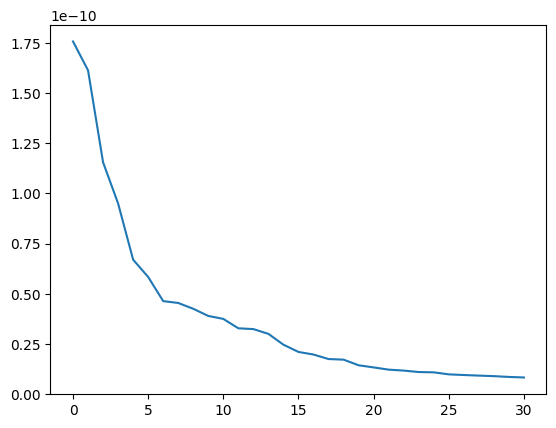
\includegraphics[width=9cm]{30vp.png}
    \caption{Graphe des 30 premières valeurs propres issues de la SVD de la matrice des données pour un sujet de la tâche visuelle}
    \label{fig4.3}
\end{figure}

Dans notre cas, cela revient à prendre les 10 premières valeurs propres. Les vecteurs propres que nous gardons correspondent aux directions selon lesquelles on retrouve le plus d'informations quand à la variabilité des valeurs des champs magnétiques au cours du temps mesurés par les capteurs. Ce sont les vecteurs propres associés aux valeurs propres qui permettent d'expliquer le plus, quantitativement parlant, la variance de nos données. Dans cet espace de moindre dimension, chaque dimension, i.e., chaque valeur singulière, correspond à des combinaisons linéaires des différents capteurs. 

\vspace{2ex}
On ne garde donc qu'une partie $d$ des vecteurs propres contenus dans $V$ de sorte à avoir une matrice $U' \in {R}^{n \times d}$. De la même manière, on crée $S' \in {R}^{d \times n}$ en tronquant $S$ et $V' \in {R}^{n \times d}$. On obtient alors notre matrice des données réduite par $M' = U'S'V'^T$.


\vspace{2ex}
On représente ces nouveaux canaux les uns en fonction des autres, pour former un espace des phases des valeurs singulières des capteurs. C'est dans ce nouvel hyperespace que l'on va déterminer l'histogramme des valeurs selon toutes les dimensions afin de déterminer la partition associée et découper cet hyperespace en autant d'intervalles que l'on souhaite avoir de symboles pour nos représentations symboliques. J'ai illustré cet méthode avec les données d'un sujet de la tâche visuelle en Figure \ref{fig4.4}. 

\begin{figure}[!ht]
    \centering
    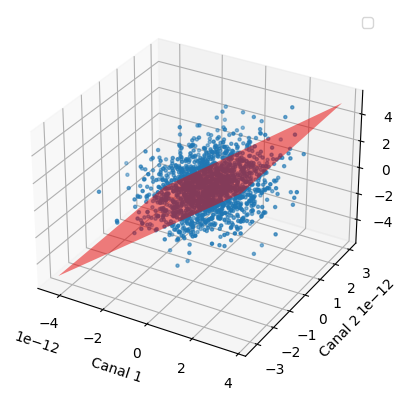
\includegraphics[width=9cm]{representation_espace_des_phases.png}
    \caption{Espace des phases de 3 valeurs singulières avec une partition binaire}
    \label{fig4.4}
\end{figure}

On récupère alors une partition selon chaque axe qui nous permet de créer nos séquences symboliques. 

\vspace{2ex}
Dans le cas où l'on fait une représentation symbolique dans l'espace des phases des données projetées sur une partie des vecteurs propres, i.e., l'espace des phases des valeurs singulières, deux choix s'offre à nous. On peut directement quantifier la dynamique de chaque séquence symbolique ou bien de créer une nouvelle séquence symbolique globale à partir des séquences symboliques obtenues. On obtient alors une séquence symbolique qui représente la dynamique globale du cerveau plutôt que par valeurs singulières, quand bien même quantifier la dynamique de chaque séquence permet d'obtenir un vecteur de taux d'entropie qui quantifie la dynamique cérébrale globale. La création d'une unique séquence symbolique résultante a du sens avec la méthode de représentation symbolique utilisée car les séquences symboliques sont représentées à partir des valeurs singulières des données, i.e., des combinaisons linéaires des capteurs. Pour se faire, on utilise la méthode recode de la classe séquence que l'on détaillera dans le chapitre suivant. Cette fonction permet de créer une séquence symbolique avec un nouvel alphabet à partir de plusieurs séquences symboliques et le fait que leur alphabet soit tous différents.
 
\vspace{2ex}
Que ce soit avec la première méthode ou la seconde, on peut ensuite quantifier la dynamique de chaque séquence symbolique et ainsi comparer la dynamique associée à différentes conditions expérimentales. C'est ce que l'on va approfondir par la suite grâce à la métrique qu'est l'entropie.

\section{Entropie}

Les éléments de la théorie de l'information présentés ci-dessous sont des résultats issus de \cite{2}. On présentera donc seulement les définitions utiles pour notre étude.
Le concept d'entropie a été définie pour la première fois par Shannon en 1948 \cite{21}. Cette quantité est une mesure de l'incertitude d'une variable aléatoire.
Soit $X$ une variable aléatoire discrète ayant $\mathcal{X}$ comme alphabet (ensemble des valeurs ou symboles que peut prendre la variable aléatoire $X$) et $p(x)=Pr\left\{X=x\right\}, x \in \mathcal{X}$ comme fonction de masse de probabilité. 
L'entropie $H(X)$ d'une variable aléatoire discrète $X$ est définie par

\begin{equation}
    H(X) = - \sum_{x \in \mathcal{X}} p(x)logp(x)
\end{equation}

Lorsqu'on s'intéresse à une seule variable aléatoire $X$, on peut aussi noter l'entropie $H(p)$ où $p$ désigne la fonction de masse de probabilité de la variable $X$.
Le $log$ est en base 2, l'unité de l'entropie est donc le bit. Il est d'usage d'également utiliser le logarithme népérien en base e pour d'autres domaines que la compression et la transmission de données. En fonction de la base du logarithme choisie, si par exemple celle-ci est $b$, on notera l'entropie associée $H_b(X)$. 

Voici quelques propriétés importantes de l'entropie :
\begin{enumerate}
    \item $H(X)\geq0$
    \item $H(p)$ est une fonction concave de p.
    \item $H_b(X)=(log_{b}a)H_{a}(X)$
\end{enumerate}

Illustrons la notion d'entropie et ses proprétés de base avec un exemple simple, celui d'un tirage aléatoire binaire \cite{8}. Comme on peut l'observer sur la Figure \ref{fig4.5}, on a $H(p)=0$ lorsque $p=0$ ou $p=1$ et $H(p)=1$ lorsque $p=1/2$. Cela revient à dire que l'entropie est nulle lorsque la variable n'est plus aléatoire (i.e. non incertaine) et que l'entropie atteint sa valeur maximale lorsque l'incertitude est maximale.

\begin{figure}[!ht]
    \centering
    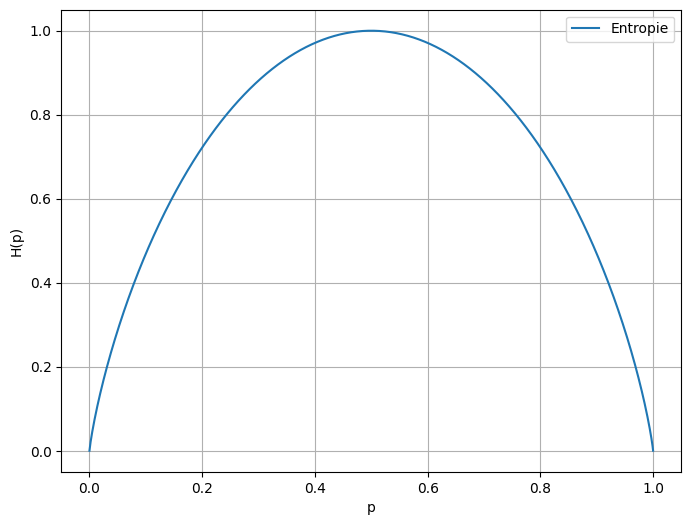
\includegraphics[width=9cm]{exemple_entropie.png}
    \caption{Entropie $H(p)$ en fonction de la probabilité $p$ d'un événement binaire}
    \label{fig4.5}
\end{figure}

En considérant une paire de variables aléatoires discrètes $(X,Y)$ de distribution joint $p(x,y)$ comme une seule variable aléatoire vectorielle, on obtient aisèment la définition de l'entropie jointe $H(X,Y)$ par

\begin{equation}
    H(X,Y) = \sum_{x \in \mathcal{X}}\sum_{y \in \mathcal{Y}}p(x, y)logp(x,y)
\end{equation}

On peut également définir l'entropie conditionnelle d'une variable aléatoire sachant une autre variable aléatoire comme la moyenne par rapport à la variable aléatoire de conditionnement des entropies des distributions conditionnelles.
Si $(X,Y) \sim p(x,y)$, alors l'entropie conditionnelle $H(Y|X)$ est donnée par 

\begin{equation}
    H(Y|X) = \sum_{x \in \mathcal{X}}p(x)H(Y|X=x) = -\sum_{x \in \mathcal{X}}p(x)\sum_{y \in \mathcal{Y}}p(y|x)logp(y|x)
\end{equation}

Ainsi, on a

\begin{equation}
    H(Y|X) = -\sum_{x \in \mathcal{X}}\sum_{y \in \mathcal{Y}}p(x,y)logp(y|x)
\end{equation}

L'entropie jointe et l'entropie conditionnelle d'une paire de variables aléatoires sont reliées par :

\begin{equation}
    H(X,Y) = H(X) + H(Y|X)
\end{equation}

Ce qui nous permet d'introduire la règle de la chaîne pour l'entropie.
Afin de pouvoir définir le taux d'entropie d'un processus stochastique dans la section suivante, on généralise la règle de la chaîne pour une collection de $n$ variables aléatoires. En effet, l'entropie d'une collection de variables aléatoires est défini par la somme des entropies conditionnelles.

Soit $X_1, X_2, ...,X_n$ une collection de variables aléatoires distribuées selon $p(x_1, x_2, ...,x_n)$. 

\vspace{2ex}
On a alors

\begin{equation}
    H(X_1, X_2, ...,X_n)= \sum_{i=1}^{n}H(X_i|X_{i-1},...,X_1) \label{eq:chaine}
\end{equation}

\vspace{2ex}
Nous allons à présent détailler notre démarche quand au calcul du taux d'entropie d'une séquence symbolique.

\section{Processus stochastique et taux d'entropie}

Les séquences symboliques extraites à partir des segments temporels des données MEG peuvent donc être considérées comme des processus stochastiques.

D'après \cite{2}, un processus stochastique $\textbf{Z}=\{Z_i \}$ est une séquence indexée de variables aléatoires. En général, il peut y avoir une dépendance arbitraire entre les variables aléatoires. Le processus est caractérisé par les fonctions de masse de probabilité conjointes

\begin{equation}
    Pr\{(Z_1, Z_2, ...,Z_n)=(z_1, z_2, ...,z_n)\}=p(z_1, z_2, ...,z_n)
\end{equation},
$(z_1, z_2, ...,z_n) \in \mathcal{Z}^n$ pour $n=1,2,...$

\vspace{2ex}
Une caractéristique importante d'un processus stochastique est la stationnarité. Un processus stochastique est dit \textit{stationnaire} si la distribution conjointe de tout sous-ensemble de la séquence de variables aléatoires est invariante par rapport aux changements de l'indice de temps ; c'est-à-dire,

\begin{equation}
    Pr\{Z_1=z_1,Z_2=z_2,..., Z_n=z_n \} = Pr\left\{Z_{1+l}=z_1,Z_{2+l}=z_2,..., Z_{n+l}=z_n \right\}
\end{equation}

Dans notre cas, on fera l'assomption que les séquences symboliques extraites des données MEG sont des processus stochastiques stationnaires. En effet, la représentation symbolique du signal en entier ne peut pas être considéré comme un processus stochastique mais il est stationnaire par morceaux, i.e. localement stationnaire. En choisissant des segments temporels courts (1.4 sec) centrés sur des événements clairement identifiés (comme par exemple l'apparition sur l'écran d'un target word lors de la tache visuelle), on peut considérer les représentations symboliques extraites de ces segments comme stationnaires.

On a vu dans la partie précédente, que l'on pouvait calculer l'entropie d'une collection de variables aléatoires $H(Z_1, Z_2, ...,Z_n)$ (5.7). On s'intéresse à la limite lorsque n tend vers l'infini de cette métrique que l'on appelle taux d'entropie. Le taux d'entropie permet de mesurer des structures de réccurence et donc la production d'information de la source, c'est l'accélération de l'entropie.
Le taux d'entropie d'un processus stochastique  $\textbf{Z}=\{Z_i \}$ est alors défini d'après \cite{2} par

\begin{equation}
    H(\textbf{Z})=\lim_{n \to \infty}\frac{1}{n}H(Z_1, Z_2, ...,Z_n) \label{eq:taux1}
\end{equation}

Quand la limite existe. 
Ce taux d'entropie correspond à la limite des entropies par symboles des variables aléatoires. 

On peut aussi définir une quantité liée pour le taux d'entropie \cite{2} d'après \eqref{eq:chaine} telle que 

\begin{equation}
    H'(\textbf{Z})=\lim_{n \to \infty} H(Z_n|Z_{n-1},Z_{n-2}...,Z_1) \label{eq:taux2}
\end{equation}

Lorsque la limite existe.
Cette deuxième notion du taux d'entropie correspond à la limite de l'entropie conditionnelle de la dernière variable aléatoire du processus stochastique sachant les états des variables aléatoires précédentes.
Pour un processus stochastique stationnaire, les limites convergent et on a égalité entre les deux taux.

\begin{equation}
    H(\textbf{Z}) = H'(\textbf{Z}) = h \label{eq:convergence1}
\end{equation}

Ce résultat est asymptotique alors que nous disposons d'un jeu de données fini et donc de séquences symboliques finies. Il en va de déterminer le taux d'entropie en utilisant un estimateur, c'est ce que nous allons présenter maintenant. 

\section{Estimateur de Lempel-Ziv}

L'ultime partie de notre algorithme est le calcul du taux d'entropie des séquences symboliques issues des séries temporelles des données MEG. Le taux d'entropie étant asymptotique et les séquences que l'on génère étants finies, on va donc utiliser un estimateur de cette quantité. Nous avons décidé d'utiliser l'estimateur de Lempel-Ziv \cite{1}. En effet, les séquences symboliques extraites à partir des époques des séries temporelles MEG contiennent 1200 symboles et la convergence de la complexité de Lempel-Ziv vers le réel taux d'entropie a été prouvée \cite{1} pour de courtes séquences, i.e., des séquences de moins de 1000 symboles. De plus, c'est un estimateur sans paramètres libres qui constitue une véritable mesure du taux d'entropie. Enfin, l'estimateur de Lempel-Ziv avait déjà été implémenté par Jean-Luc Blanc et Laurent Pezard dans le module scikits-symbolic. C'est pour ces raisons que nous avons choisi d'utiliser cet estimateur du taux d'entropie. Nous allons à présent expliquer son fonctionnement.

\vspace{2mm}
Considérons une source stationnaire qui émet à chaque pas de temps un symbole d'un alphabet de taille finie $k$. Son entropie de bloc d'ordre $n$ est définie comme l'entropie de Shannon de la distribution de probabilité $p_n(w)$ des mots de longueur $n$ (i.e. des mots de n symboles),

\begin{equation}
    H_n = - \sum_{w}p_n(w)lnp_n(w)
\end{equation}

\begin{enumerate}
	\item $w$ mot de longueur n
	\item $p_n(w)$ distribution de probabilité
\end{enumerate}

Cette somme est calculée sur tous les mots de longueur $n$ possibles $w$, et dépend donc de la dynamique de la source sur les $n$ intervalles de temps.
En conséquence, $h_n = H_{n+1} - H_n$ converge vers une limite $h$ lorsque la longueur des mots tend vers $\infty$, ce qui correspond au taux d'entropie de la source.

\begin{equation}
    h = \lim_{n \to \infty}\frac{H_n}{n} = \lim_{n \to \infty}H_{n+1} - H_n \label{eq:convergence2}
\end{equation}

Ces deux définitions du taux d'entropie correspondent dans l'ordre aux définitions établis en \eqref{eq:taux1} et en \eqref{eq:taux2} d'après \cite{2}. Les équations \eqref{eq:convergence1} et \eqref{eq:convergence2} sont donc équivalentes.

\vspace{2ex}
En pratique, le taux d'entropie $h$ doit le plus souvent être estimé à partir d'une seule séquence observée $[s] = (s_i)_{1 \geq i \geq N}$ de longueur $N$. 
Nous désignerons dorénavant $\hat{X}$ comme l'estimateur d'une quantité $X$, sans mentionner explicitement qu'il dépend de la séquence $[s]$ et de sa longueur $N$. Regarder la limite du taux d'entropie lorsque $n$ tend vers l'infini revient à observer la limite de cette même quantité lorsque $N$ tend vers l'infini.

\vspace{2ex}
Le point de vue adopté pour calculer la complexité de Lempel-Ziv est a priori très différent de celui associé au taux d'entropie de Shannon $h$. En effet, la définition du taux d'entropie de Shannon $h$ implique une caractéristique globale de la dynamique, à savoir sa mesure invariante. Elle peut être calculée à partir de la connaissance d'une seule trajectoire tant que la mesure est ergodique et permet de reconstruire la distribution de probabilité de la source à partir de l'observation d'une seule séquence typique. Mais elle n'est pas, en soi, significative en tant que caractéristique d'une séquence unique. En revanche, la complexité de Lempel-Ziv fournit une mesure de la compressibilité de la séquence symbolique unique considérée, en d'autres termes, le contenu de l'information par symbole. Dans l'hypothèse où la source est stationnaire et ergodique, les théorèmes de Lempel-Ziv \cite{16} garantissent que la complexité de Lempel-Ziv coïncide avec $h$ jusqu'à un facteur $lnk$ impliquant le nombre $k$ de symboles de l'alphabet (la partition utilisée) comme défini en \eqref{eq:lempelziv}. Cette hypothèse implique en effet que presque toutes les séquences symboliques ont les mêmes caractéristiques de compressibilité ; le calcul peut donc être effectué de manière équivalente avec n'importe quelle séquence typique et son résultat coïncide avec la moyenne.

Selon le schéma de Lempel-Ziv, la séquence de longueur $N$ est découpée en $\mathcal{N}_w$ mots. Deux manière de découper la séquence et donc de construire le dictionnaire de mots ont été proposées. On utilisera la première manière de créer des mots à partir des symboles de la séquence, publié en 1976 \cite{15}, qui considère comme mot le plus court ensemble de symboles qui n'a pas encore été rencontré lors du balayement de la séquence. Par exemple :

\begin{equation}
    1 \cdot 0 \cdot 01 \cdot 11 \cdot 100 \cdot 101 \cdot 00 \cdot 010 \cdot 11... .
\end{equation}

Une fois le dictionnaire de mots construit à partir de la séquence, on calcule 

\begin{equation}
    \hat{L} = \frac{\mathcal{N}_w[1 + log_k\mathcal{N}_w]}{N}
\end{equation}

où

\begin{equation}
    \lim_{n \to \infty} \hat{L} = \frac{h}{lnk} \label{eq:lempelziv}
\end{equation}

\begin{enumerate}
	\item $k$ taille de l'alphabet
	\item $\mathcal{N}_w$ nombre de mots du dictionnaire
	\item $N$ taille de la séquence symbolique
\end{enumerate}

C'est donc de cette manière que nous avons calculé la complexité de Lempel-Ziv $\hat{L}$, qui nous donne une très bonne estimation du taux d'entropie d'une séquence symbolique. L'algorithme de Lempel-Ziv que nous avons utilisé fait partie du module scikits-symbolic sur lequel j'ai apporté une contribution et que je vais présenter dans le prochain chapitre.

\chapter{Développement et code Python}

\section{Scikits-symbolic}

\vspace{2ex}
Dans cette section, nous allons décrire l'implémententation des approches de la théorie de l'information pour pouvoir appliquer notre algorithme sur les données MEG. Pour se faire, j'ai travaillé sur un module initialement développée par Jean-Luc Blanc et Laurent Pezard il y a quelques années. Nous avons travaillé de manière collaborative en utilisant le logiciel GitLab. Le Git du module scikits-symbolic est disponible à cette adresse \href{http://git.lnc.dcs.univ-amu.fr/lpezard/scikits-symbolic/}{http://git.lnc.dcs.univ-amu.fr/lpezard/scikits-symbolic/}.

\vspace{2ex}
Le module scikits-symbolic est un ensemble de fonctions, de classes et de méthodes de la théorie de l'information permettant de manipuler les séquences symboliques. En effet, j'ai utilisé le module scikits-symbolic pour représenter symboliquement la dynamique cérébrale en déterminant des séquences symboliques à partir des canaux du signal MEG et d'en calculer leur taux d'entropie. C'est donc dans cette perspective que j'ai alimenté le code déjà existant.

\vspace{2ex}
J'ai donc travaillé avec Laurent Pezard sur le scikits-symbolic afin d'obtenir une version stable en y ajoutant les tests nécessaires pour pouvoir le publier en tant que Scikit. Ce travail m'a permis de manipuler des métriques issus de la théorie de l'information en lien avec mon sujet telles que les séquences symboliques, les fonctions de partition et de représentation symbolique dans l'espace des phases. J'ai donc pu affiner ma compréhension des outils que j'ai par la suite utilisé lors de mon stage.

\vspace{2ex}
Toutefois, l'objectif de mon travail sur ce module était essentiellement d'implémenter une batterie de tests sur les scritps pour vérifier et prouver leur bon fonctionnement. Nous détaillerons plus tard cet aspect dans la partie dédiée.

\section{Structure et classes}

L'arborescence principale du scikits-symbolic est présentée en Figure \ref{fig5.1}.

\begin{figure}[!ht]
    \centering
    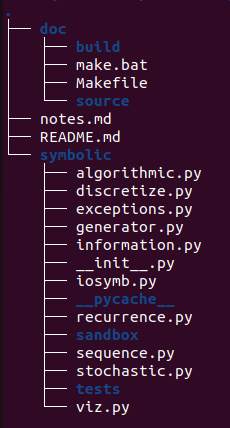
\includegraphics[width=4cm]{arborescence.png}
    \caption{Arborescence (de profondeur 2) du module scikits-symbolic}
    \label{fig5.1}
\end{figure}

\vspace{2ex}
On affiche ici seulement les principaux fichiers .py sans expliciter le contenu des autres répertoires. Toutefois, il est important de noter que le module est également composée de fichiers .rst dans les répertoires souce et build permettant la création de la documentation via Sphinx, que l'on détaillera plus tard, ainsi que d'autres fichiers sous-jacents permettant le fonctionnement du module scikits-symbolic. On va ici présenter seulement les différents fichiers sur lesquels j'ai apporté une contribution.

\vspace{2ex}
Le fichier central de scikits-symbolic est sequence.py où sont définis les différentes classes ainsi que leurs méthodes associées. Il y a 3 classes différentes, la classe State permet de définir un état. On peut créer un état, celui-ci représente et constitue le lien entre un entier et un symbole (qui peut-être une lettre d’un alphabet). 

\vspace{2ex}
La seconde classe est l’Alphabet. L’alphabet est une liste d’état, il peut être créé à partir d’une liste de States définis préalablement ou bien en donnant simplement le nombre de symboles que l’on souhaite dans notre alphabet. Cet objet  constitue une des deux bases indispensables à la définition d’une représentation symbolique. En effet, l’alphabet permet de conserver la représentation de la dynamique symbolique comme un vecteur de nombres entiers (facilement manipulable pour des calculs de la théorie de l’information) tout en ayant le lien visible avec la signification de chaque entiers de par leur association avec les symboles de l’alphabet. 

\vspace{2ex}
La dernière classe qui est au centre de nos intérêts et constitue la pièce centrale du scikit est donc l’objet Sequence qui permet de définir informatiquement une séquence symbolique. On voit donc que ces 3 classes sont imbriquées les unes dans les autres. La définition d’un objet séquence symbolique nécessite un vecteur qui est la séquence d’entier ainsi qu’un alphabet. Et la création d’un alphabet nécessite la définition des différents States qui le constituent.
De cette manière, la classe sequence permet d'avoir un objet informatique contenant toutes les propriétés et informations nécessaires pour correspondre au concept de séquence symbolique et donc à sa définition mathématique. 
Les méthodes implémentées pour la classe sequence permettent donc en autres d'obtenir la taille d'une séquence symbolique ainsi que la taille de son alphabet, de calculer son entropie de Shannon, etc. Il est également possible de créer une séquence symbolique à partir de deux séquences symboliques à condition qu'elles soient de même taille grpave à la fonction recode. Cela est possible pour deux séquences symboliques ayant des alphabets différents et même de taille différente. Cette fonction crée donc un nouvel alphabet qui prend en compte les symboles contenu dans les alphabets d'origine. Comme expliqué dans la partie 4.2.2, c'est une fonction que l'on a utilisé pour obtenir une séquence symbolique globale à partir de séquences symboliques représentées dans l'espace des phases de séries temporelles singulières des capteurs (projetés après une SVD). Cette séquence symbolique permet alors de rendre compte de la dynamique cérébrale globale.

\section{Fonctions}

Le reste du scikit est un ensemble de fonctions et de méthodes permettant de manipuler et de faire des opérations et des calculs au sens de la théorie de l’information sur des séquences symboliques que nous présentons ici :

\begin{enumerate}
    \item algorithmic : contient les différentes versions de l'estimateur du taux d'entropie de Lempel-Ziv;
    \item stochastic : permet le calcul des matrices de transition, matrices conditionnelles et d'influence de deux séquences symboliques qui représentent des processus stochastiques;
    \item information : permet le calcul de de différentes métriques issues de la théorie de l'information. Parmis celles-ci, on pourra citer l'information mutuelle de deux séquences symboliques ou plus, l'entropie de Shannon, etc;
    \item discretize : contient les fonctions permettant l'extraction de séquences symboliques à partir de séries temporelles
\end{enumerate}

\vspace{2ex}
Les fonctions du fichier discretize correspondent aux implémentations des méthodes de représentation symbolique explicitées dans la partie 4.2.

\section{Tests sur le scikits et documentation associée}

\vspace{2ex}
La convergence et les fondements théoriques des différents codes du module scikits-symbolic sur lesquels j'ai effectué les tests ont déjà été prouvés. Mon travail était donc de vérifier la correction des différents algorithmes. J'ai implémenté les tests directement sur le code, grâce au module Doctest qui permet d'écrire un test directement dans la définition de la fonction ou de la classe. On écrit les tests entre guillements, comme si l'on écrivait dans un document texte. En effet, le module Doctest permet d'écrire des prompts de commande que l'ordinateur va éxecuter lorsque qu'il va run le code. Comme on peut le voir en Figure \ref{fig5.3}, on écrit des commandes comme si les écrivait directement dans un shell Python avec ">>>" en amont pour indiquer une requête. Les lignes sans ">>>" correspondent à ce qu'est censé renvoyé l'ordinateur lors de la lecture des commandes, ici 0.6. On peut donc lui faire exécuter une suite de commandes qui utilisent les fonctions et les objets du module scikits-symbolic sur un exemple dont on connaît déjà le résultat. De cette manière, on vérifie que l'implémentation des scripts qui composent le module a été correctement effectuée et que l'algortithme produit les résultats attendus. C'est la vérification informatique de la correction de l'algorithme. Si la sortie est égale avec ce que l'ordinateur a calculé en suivant notre suite de commande, alors le test est concluant et aucun messages d'erreur ne s'affiche. Par contre, si le résultat obtenu est différent de ce qui est censé être trouvé, un message d'erreur s'affiche et cela permet de mettre en exergue un mauvais fonctionnement du code qui ne fait pas ce que l'on voudrait qu'il fasse (Figure \ref{fig5.3}).

\begin{figure}[!ht]
    \centering
    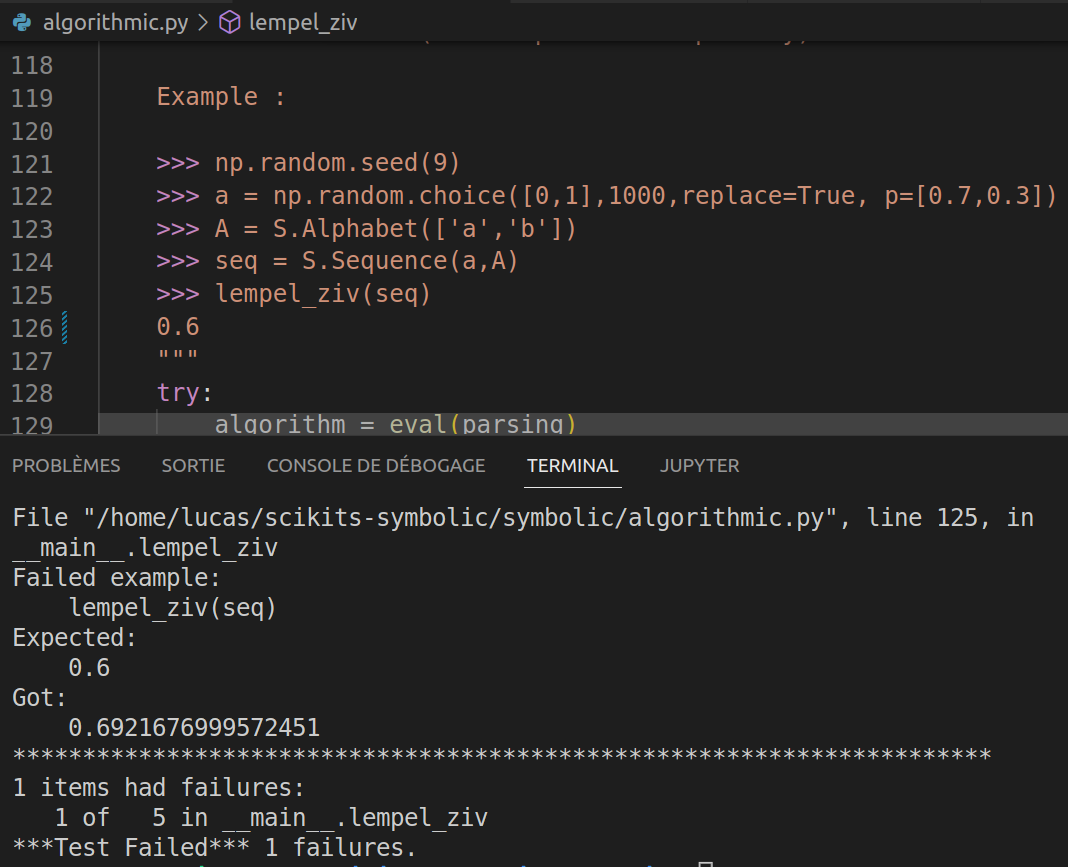
\includegraphics[width=13cm]{exemple_doctest.png}
    \caption{Exemple d'un test réalisé avec Doctest échoué. Expected représente ce que l'on a indiqué comme étant la sortie de notre ligne de commande "lempel-ziv(seq)", i.e., ce qu'est censé obtenir l'ordinateur lorsqu'il run le script en question. J'ai volontairement mis un résultat érroné pour pouvoir afficher le message d'erreur d'un test echoué. Got correspond au résultat effectivement obtenu par l'ordinateur lors de la lecture du script.}
    \label{fig5.3}
\end{figure}

\vspace{2ex}
Cette manière de tester en écrivant directement dans la définition d'une classe ou d'une fonction allait de paire avec la création d'une documentation pour le scikits-symbolic. En effet, le générateur de documentation Python Sphinx permet de générer facilement une documentation en prenant les informations contenues dans la définition d'une classe ou d'une fonction. Il suffit alors de décrire ce que fait notre code, de renseigner les différents paramètres avec une certaine typologie, d'écrire les test Doctest, tout cela au même endroit dans le code. Quelques manipulations des outils apportés par Sphinx nous permettent ensuite de générer un document pdf ou bien une page html en décidant de la structure. La documentation est consultable en deuxième partie de l'Annexe.

\chapter{Résultats}

\section{Tests d'indépendance statistique}

Je présente ici les résultats obtenus en utilisant la méthode de représentation symbolique par canaux, pour deux sujets, un de la tâche visuelle et un de la tâche auditive, selectionnés de manière aléatoire. Pour chaque ensemble d'époques relatives à une condition expérimentale, on extrait des représentations symboliques dont on estime le taux d'entropie grâce à l'estimateur de Lempel-Ziv. On obtient alors une matrice contenant le taux d'entropie les séquences symboliques extraites à partir de segments temporels d'intérêt des canaux du signal MEG (ce sont les lignes de la matrice) et ce pour chaque époque (colonnes). Pour chaque canal, on calcule la médiane sur les époques que l'on garde. On a alors un vecteur contenant les taux d'entropie relatifs à chaque canal.

\vspace{2ex}
On décide d'effectuer des tests-t statistiques \cite{22} entre les vecteurs d'entropie associés à des conditions expérimentales différentes. Par exemple, on va comparer la mesure obtenue sur les target words au sein des phrases avec celle obtenue sur les target words au sein des listes aléatoires de mots.
Le test-t nous donne un résultat important, il nous informe si la différence observée entre les deux mesures est statistiquement significative.

\vspace{2ex}
Etant donné que nos mesures proviennent du même sujet, même s'il a été soumis à des stimuli différents, on peut donc considéré nos vecteurs d'entropie comme appariés. En effet, le test-t pour échantillons appariés peut être utilisé pour des sujets qui ont été exposés à deux conditions expérimentales. Les quantités que l'on compare sont des taux d'entropie qui constituent bien une mesure au sens mathématique du terme et l'on a utilisé la même métrique pour chaque condition expérimentale. 

\section{Interprétation des résultats}

On s'intéresse à la valeur p ou "p-value" comme résultat du test-t. Celle-ci nous donne la probabilité de l'hypothèse nulle, i.e., que les deux populations sont statistiquement identiques. Lorsque l'on obtient une valeur p inférieure à $5\%$, $p\geq 0.05$, on peut considérer que la probabilité de l'hypothèse nulle correspond au hasard et donc que les deux échantillons sont statistiquement différents.

On présente ici les résultats que nous avons obtenus en comparant les échantillons de taux d'entropie relatifs à différentes conditions expérimentales.

\subsection{Target word vs individual word}

\begin{figure}[!ht]
    \centering
    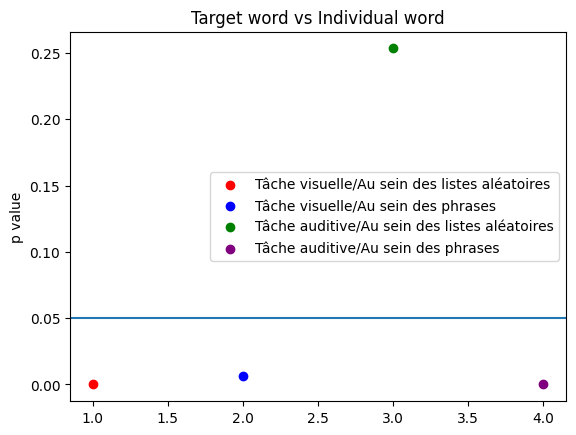
\includegraphics[width=10cm]{Targetword_vs_Individualword.png}
    \caption{Tests t apparayés entre les vecteurs d'entropie relatifs aux target words par rapport aux individual words}
    \label{fig6.1}
\end{figure}

On observe que pour la tâche visuelle, les dynamiques cérébrales associées aux target words et aux individual words sont statistiquement différentes, que ce soit au sein des phrases ou des listes aléatoires de mots. Pour la tâche auditive, les dynamiques cérébrales associées aux targets words et aux individual words sont statistiquement différentes au sein des phrases tandis qu'elles sont statistiquement différentes au sein des listes aléatoires de mots. On peut donc confirmer que pour la tâhce auditive, la dynamique cérébrale permet effectivement de distinguer des degrés de complexité linguistiques en lien avec des conditions expérimentales différentes.

\subsection{Phrases simples vs listes aléatoires de mots issues de phrases simples}

\begin{figure}[!ht]
    \centering
    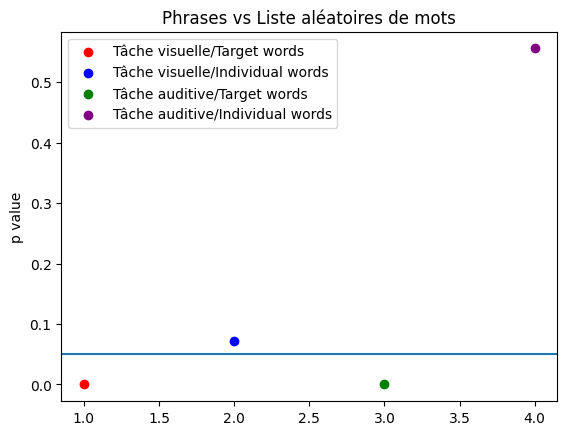
\includegraphics[width=10cm]{Phrases_vs_Listes_aleatoires.png}
    \caption{Tests t apparayés entre les vecteurs d'entropie relatifs aux phrases par rapport aux listes aléatoires de mots}
    \label{fig6.2}
\end{figure}

On retrouve ici ce que l'on a pu observer sur le graphique de résultats précédent. En effet, les target words semblent être les piliers de compréhension des phrases, ce qui permet d'indexer la complexité linguistique avec la dynamique cérébrale. En effet, les mesures de la dynamique cérébrale sont statistiquement différentes entre les phrases simples et les listes aléatoires de mots lorsque l'on s'intéresse aux targets words. Ce n'est pas le cas lorsque l'on se base sur les individual words, où les dynamiques cérébrales associées sont statistiquement semblables.

\subsection{Tâche visuelle vs tâche auditive}

\begin{figure}[!ht]
    \centering
    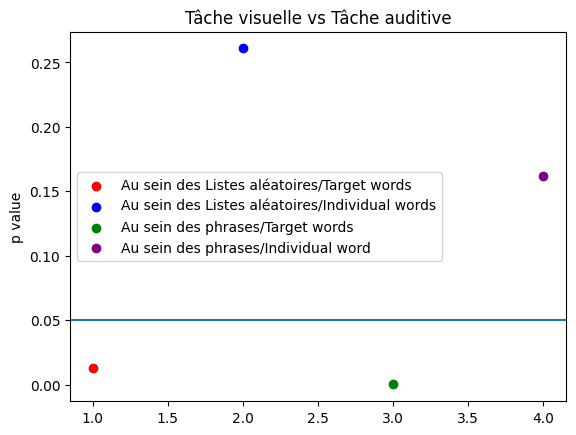
\includegraphics[width=10cm]{visuelle_vs_auditive.png}
    \caption{Tests t apparayés entre les vecteurs d'entropie relatifs à la tâche visuelle par rapport par rapport à la tâche auditive}
    \label{fig6.3}
\end{figure}

On observe que les dynamiques cérébrales associées à la tâche visuelle et auditive sont statistiquement différentes lorsque l'on se base sur les target words, que ce soit au sein des phrases ou bien des listes aléatoires de mots. Encore une fois, la compréhension linguistique auditive et visuelle ne s'opérant pas de la même manière, on peut les discriminer grâce à la dynamique cérébrale en se basant sur les target words, que ce soit au sein des phrases ou des listes aléatoires de mots. Comme on pouvoit s'y attendre, cette conclusion n'est pas possible lorsque l'on s'intéresse aux individual word. En effet, les dynamiques associées sont statistiquement semblables dans la tâche auditive comme dans la tâche visuelle.

\subsection{Récapitulatif des résultats des tests statistiques}

\begin{figure}[!ht]
    \centering
    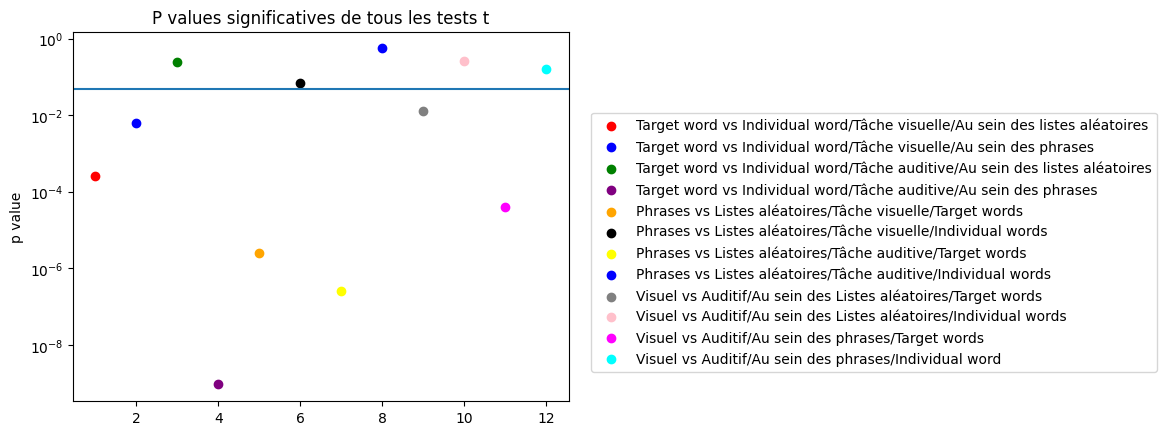
\includegraphics[width=15cm]{p_value_significative.png}
    \caption{Valeurs p significatives des tests t. L'axe des ordonnées est en échelle logarithmique afin de pouvoir distinguer les différentes valeurs}
    \label{fig6.4}
\end{figure}

On peut conclure qu'avec la démarche scientifique que l'on a appliqué et la segmentation temporelle effectuée, le taux d'entropie est majoritairement un bon indicateur pour indexer le complexité linguistique. Toutefois, la dynamique cérébrale ne permet pas de discriminer des conditions expérimentales à chaque fois.

\chapter*{Conclusion}
\addcontentsline{toc}{chapter}{Conclusion}

A travers le travail que j'ai mené durant mon stage, j'ai pu appliquer une démarche méthodologique basée sur la théorie de l'information et la théorie des systèmes dynamiques. Grâce à la représentation symbolique et sur la base de signaux MEG qui constituent une mesure de l'activité cérébrale, j'ai réussi mettre en exergue le lien entre dynamique cérébrale et complexité linguistique en utilisant comme métrique l'entropie. En effet, dans le contexte où on l'a utilisé, la représentation symbolique permet la majeure partie du temps de caractériser un système dynamique continu (le cerveau) comme une séquence de symboles correspondants à des états discrets. Cela permet de rendre compte de la complexité intrinsèque de la dynamique cérébrale et de la quantité d'information contenue dans celle-ci grâce à l'entropie. Le taux d'entropie comme résultat final de l'algorithme mis en place durant le stage semble être un bon indicateur de la complexité linguistique et a permis de discriminer des conditions expérimentales à partir des mesures de l'activité cérébrale. 

Comme perspectives futures, il serait intéressant d'appliquer une segmentation temporelle différente et s'intéresser à la variation du taux d'entropie au cours d'une phrase. Aussi, il faudrait appliqué l'algorithme développé au cours du stage sur l'ensemble des 204 sujets de la base de données MOUS. En effet, de par la variabilité interindividuelle, il serait intéressant de mener l'étude sur une plus grande quantité de sujets différents. Cela permettrait de réduire encore plus le rapport signal sur bruit et obtenir des résultats plus robustes. On notera aussi qu'il existe des méthodes de représentation symbolique plus complexes qui permettent de rendre compte plus en détails de la dynamique cérébrale. En effet, la décomposition atomique \cite{7} est une méthode de représentation symbolique qui consiste à extraire des atomes spatio-temporels du signal. Cette manière plus fine de représenter symboliquement un système dynamique pourrait être une des pistes de développement futur du projet.


\bibliography{biblio.bib}
\addcontentsline{toc}{chapter}{Bibliographie}

\renewcommand{\appendixpagename}{Annexes}
%\renewcommand{\appendixtocname}{Annexes}
\appendix
\appendixpage
\addappheadtotoc
\section*{Séquence symbolique}

Cette partie a été adaptée de \cite{3}.

\subsection*{Partitions}

Soit $(\Omega,\mathcal{B},\mu)$ un espace mesuré, i.e $\Omega$ est un ensemble non-vide appelé l'espace des états, $\mathcal{B}$ est une tribu de sous-ensembles de $\Omega$, et $\mu$ est une mesure positive sur l'espace mesurable $(\Omega,\mathcal{B})$. Une partition de $\Omega$ est une famille disjointe d'éléments de $\mathcal{B}$, non-vides et dont l'union est $\Omega$.
On suppose que $\mu(\Omega) \geq\infty$, on peut alors dire que $(\Omega,\mathcal{B},\mu)$ est un espace de probabilité i.e. $\mu(\Omega)=1$.
On considérera par la suite essentiellement des partitions finies, i.e. une partition avec un nombre fini d'éléments qui ont une mesure positive. La Figure \ref{fig7.1} illustre un exemple d'une partition finie.

\begin{figure}[!ht]
    \centering
    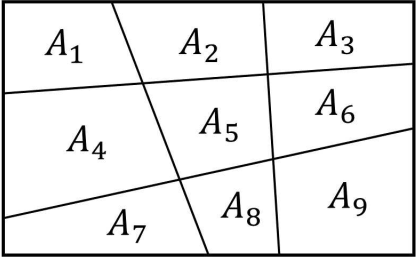
\includegraphics[width=10cm]{illustration_partition.png}
    \caption{Un domaine rectangulaire du plan est divisé en 9 sous-ensembles disjoints $A_1, A_2,..., A_9$ (extrait de \cite{3})}
    \label{fig7.1}
\end{figure} 

\vspace{2ex}
Les partitions seront représentées par des lettres grecques minuscules. On introduit la partition de points distincts qui nous servira dans la partie sur les partitions génératrices :

\begin{equation}
    \epsilon = \left\{\left\{x\right\} : x \in \Omega \right\}
\end{equation}

\vspace{2ex}
Soit $\alpha = \left\{A_1,..., A_{|\alpha|}\right\}=\left\{A_a : 1 \geq a \geq |\alpha|\right\}$ et $\beta = \left\{B_1,..., B_{|\beta|}\right\}=\left\{B_a : 1 \geq a \geq |\beta|\right\}$ des partitions de $\Omega$, où $|\alpha|$ désigne le cardinal de l'ensemble $\alpha$.

\vspace{2ex}
On défini la partition $\alpha \lor \beta = \left\{A_a \cap B_b : 1 \geq a \geq |\alpha|, 1 \geq b \geq |\beta|\right\}$ comme le raffinement de $\alpha$ et $\beta$. La raffinement de plus de deux partitions est défini de manière récursive.

\vspace{2ex}
L'entropie de $\alpha$ est définie par

\begin{equation}
    H_{\mu}(\alpha) = - \sum_{a=1}^{|\alpha|}\mu(A_a)log_{\mu}(A_a)
\end{equation}

où le logarithme peut être en base 2 ou e.

\vspace{2ex}
Si $X : \Omega \longrightarrow \left\{1,...,|\alpha|\right\}$ est une variable aléatoire définie par $X(\omega) = a$ si et seulement si $\omega \in A_a$, alors $H_\mu(\alpha)$ coïncide avec l'entropie de Shannon de $X$,

\begin{equation}
    H(X) = - \sum_{a=1}^{|\alpha|}Pr\left\{X=a\right\}logPr\left\{X=a\right\}
\end{equation}

puisque la probabilité que $X=a$ est $Pr\left\{X=a\right\}=\mu\left\{X^{-1}(a)\right\}=\mu(A_a)$.

Comme vu précédemment, $H(X)$ mesure l'incertitude des valeurs prises par la variable aléatoire $X$.

\subsection*{Système dynamique et entropie}

\vspace{2ex}
Une fois que les espaces de probabilité et les partitions ont été introduits, l'ingrédient restant est le concept de dynamique ou de passage du temps.
Considérons un espace probabilisé $(\Omega,\mathcal{B},\mu)$ comme défini précédemment ainsi qu'une application mesurable $f : \Omega \longrightarrow \Omega$, i.e., $f^{-1}(B) \in \mathcal{B}$ pour tout $B \in \mathcal{B}$. Le lien entre l'espace de probabilité et l'application mesurable réside dans le fait que $f$ préserve la mesure, i.e. $\mu(f^{-1}(B))=\mu(B)$ pour tout $B \in \mathcal{B}$. Alternativement, on dit que $f$ est $\mu$-invariant ou bien que la mesure $\mu$ est $f$-invariante. En particulier, si on prend une partition $\alpha =\left\{A_a : 1 \geq a \geq |\alpha|\right\}$ de $\Omega$, alors $f^{-1}(\alpha) =\left\{f^{-1}(A_a) : 1 \geq a \geq |\alpha|\right\}$ est aussi une partition de $\Omega$.
Si, de plus, $f$ est une application préservant la mesure, un à un, et que $f^{-1}$ préserve également la mesure, alors on dit que $f$ est une application inversible préservant la mesure.

\vspace{2ex}
En s'appuyant sur les définitions précédentes, on appelle $(\Omega, \mathcal{B}, \mu, f)$ un système dynamique (préservant la mesure). Les dynamiques de ce système sont générées par les itérations $f^{n+1}(x) = f(f^n(x))$ au pas de temps discrets $n \in \mathbb{T}$. La séquence $(f^n(x))_{n \in \mathbb{T}}$ est appelée orbite ou trajectoire avant (resp. complète) de $x$ si $\mathbb{T} = \mathbb{N}_0$ (resp. $\mathbb{T} = \mathbb{Z}$); $x$ est parfois appelé la condition initiale.

\vspace{2ex}
A ce stade et pour la suite, il nous faut introduire une définition. Il est dit que $(\Omega_1,\mathcal{B}_1,\mu_1,f_1)$ et $(\Omega_2,\mathcal{B}_2,\mu_2,f_2)$ sont isomorphes s'il existe $M_i \in \mathcal{B}_i (i=1,2)$ avec $\mu(M_i)=1$ et $f(M_i) \subset M_i$, et qu'il existe une application inversible préservant la mesure$\Phi: M_1 \longrightarrow M_2$ avec $(\Phi \circ f_1)(x)=(f_2 \circ \Phi)(x)$, $\forall x \in M-1$. L'application $\Phi$ est appelée un isomorphisme.

\vspace{2ex}
Si l'on considère le système dynamique à mesure preservée $(\Omega,\mathcal{B},\mu,f)$ et une partition $\alpha = \left\{A_a : 1 \geq a \geq |\alpha|\right\}$ de $(\Omega,\mathcal{B},\mu)$, alors  

\begin{equation}
    h_{\mu} = \lim_{n \to \infty} \frac{1}{n} H_{\mu}(\bigvee_{i=0}^{n-1} f^{-i}\alpha)
\end{equation}

Est appelée l'entropie de f par rapport à la partition $\alpha$. Avec l'équation (5.7), on obtient

\begin{equation}
    H_{\mu}(\bigvee_{i=0}^{n-1} f^{-i}\alpha) = \sum_{a_0,a_1,...,a_{n-1}} \mu(A_{a_0} \cap f^{-1}A_{a_1} \cap...\cap f^{-n+1}A_{a_{n-1}})log\mu(A_{a_0} \cap f^{-1}A_{a_1} \cap...\cap f^{-n+1}A_{a_{n-1}})
\end{equation}

On peut à présent introduire l'entropie de Kolmogorov-Sinai de l'application f avec le même système dynamique à mesure preservée que précédemment $(\Omega,\mathcal{B},\mu, f)$. Celle-ci est définie de la manière suivant

\begin{equation}
    h_{\mu}(f) = sup h_{\mu}(f,\alpha)
\end{equation}

où le supremum est pris sur toutes les partitions finies de $(\Omega,\mathcal{B},\mu)$.  On verra par la suite que le supremum est atteint pour des partitions génératrices dans l'espace des phases (états).

\subsection*{Dynamique symbolique par rapport à une partition}

\vspace{2ex}
On a vu que tout processus aléatoire stationnaire à temps discret sur un espace de probabilité correspond à un système dynamique préservant la mesure.

\vspace{2ex}
En effet, soit $Z = \left\{Z_n\right\}_{n \in \mathbb{T}}$ un processus aléatoire (i.e. stochastique) sur un espace de probabilité $(\Omega,\mathcal{B},\mu)$ avec comme états $\left\{1,...,k\right\}$ et une distribution jointe de probabilité $p(z_{n_1},...,z_{n_r})$ où $r \geq 1$ et $z_{n_1},...,z_{n_r} \in \left\{1,...,k\right\}$. On note $\left\{1,...,k\right\}\}^\mathbb{T}$ l'ensemble de toutes les séquences ayant comme symboles $\left\{1,...,k\right\}$. On définit l'application de codage mesurable $\Phi : \Omega \longrightarrow \left\{1,...,k\right\}$ tel que $\Phi(\omega) = (Z_n(\omega))_{n \in \mathbb{T}}$ et $\mathcal{C}$ la tribu produit générée par les ensembles cylindriques, i.e. les ensembles des séquences à valeurs dans $\left\{1,...,k\right\}^\mathbb{T}$ avec un nombre fini de composantes fixées. En outre, on dote l'espace mesurable $(\left\{1,...,k\right\}^\mathbb{T}, \mathcal{C})$ d'une mesure transportée $m = \mu \circ \Phi^{-1}$, i.e.,

\begin{equation}
    m(C) = \mu(\Phi^{-1}C), C \in \mathcal{C}
\end{equation}

de sorte à ce que $\Phi$ préserve la mesure. 

L'opérateur de décalage $\sigma : (z_n)_{n \in\mathbb{T}} \longrightarrow (z_{n+1})_{n \in \mathbb{T}}$ sur l'espace de probabilité $(\left\{1,...,k\right\}\}^\mathbb{T}, \mathcal{C},m)$ est alors $m$-invariant de par la stationarité de $Z$.
On a alors $(\left\{1,...,k\right\}\}^\mathbb{T}, \mathcal{C}, m, \sigma)$ qui constitue un système dynamique préservant la mesure que l'on appelle système dynamique discret ou support de $Z$, $Supp(Z)$.
Les états du système dynamique $Supp(Z)$ sont les trajectoires ou réalisations $(z_n)_{n \in \mathbb{T}}$ du processus aléatoire $\textbf{Z}$. Si $n=0$ correspond au temps actuel, les valeurs de $\textbf{Z}$ sont mis à jour grâce à l'application de décalage $\sigma$.

Comme vu dans les parties précédentes, le taux d'entropie de Shannon du processus stochastique stationnaire $\textbf{Z}=\left\{Z_n\right\}_{n\in\mathbb{T}}$, avec comme états $(\left\{1,...,k\right\}\}$, est défini par

\begin{equation}
    h(\textbf{Z})=-\lim_{n \to \infty}\sum_{z_1,...,z_n}Pr\left\{Z_1=z_1, ...,Z_n=z_n\right\}logPr\left\{Z_1=z_1, ...,Z_n=z_n\right\}
\end{equation}

Cette limite converge car le processus stochastique $\textbf{Z}$ est stationnaire. 

\vspace{2ex}
Nous venons de voir que tout processus aléatoire stationnaire peut être associé à un système dynamique appelé son support. Cette association est rendue possible par l'application de codage $\Phi$. Il se trouve que ce qui nous intéresse dans notre étude est le corrolaire : tout système dynamique peut être associé à un processus stochastique stationnaire avec un nombre d'états fini appelé dynamique symbolique. Cette seconde association est rendue possible par les partitions, c'est ce que l'on va expliciter par la suite.

\vspace{2ex}
On reprend le système dynamique à mesure preservée $(\Omega,\mathcal{B},\mu,f)$ et une partition $\alpha = \left\{A_a : 1 \geq a \geq |\alpha|\right\}$ de $(\Omega,\mathcal{B},\mu)$ introduit.e.s. On définit, pour tout $n \in \mathbb{T}$, l'application mesurable $Z_n^{\alpha}: \Omega \longrightarrow \left\{1,...,|\alpha|\right\}\}$ telle que

\begin{equation}
    Z_n^{\alpha}(x)=a_n \iff f^n(x)\in A_{a_n}
\end{equation}

Alors $\textbf{Z}^{\alpha}=\left\{Z_n^{\alpha}\right\}_{n\in\mathbb{T}}$ est un processus stochastique stationnaire. En effet, la distribution de probabilité jointe de $\textbf{Z}^{\alpha}$ nous est donnée par le biais de la mesure de probabilité $\mu$

\begin{equation}
    Pr \left\{ Z_0^{\alpha}=a_0, ...,Z_n^{\alpha}=a_n \right\} = \mu \left\{ x \in \Omega :x \in A_{a_0},f(x) \in A_{a_1},...,f^n(x) \in A_{a_n}\right\} = \mu\left\{A_{a_0} \cap f^{-1}A_{a_1} \cap...\cap f^{-n}A_{a_n}\right\}
\end{equation}

La stationnarité de $\textbf{Z}$ est triviale de par le fait que $\mu$ soit $f$-invariant.

\vspace{2ex}
La séquence $(a_n)_{n\in\mathbb{T}}$ constitue la trajectoire symbolique de $x$ par rapport à la partition $\alpha$, $a_n \in \left\{1,...,|\alpha|\right\}$ étant le nième symbole de la trajectoire.

\vspace{2ex}
$\textbf{Z}^{\alpha}=\left\{Z_n^{\alpha}\right\}_{n\in\mathbb{T}}$ défini dans l'équation (3.19) est la dynamique symbolique de $f$ par rapport à la partition $\alpha$. On en déduit de l'équation (3.20) que

\begin{equation}
    h(\textbf{Z}^{\alpha})=h_{\mu}(f,\alpha)
\end{equation}

C'est l'entropie de Kolmogorov-Sinai de l'application $f$ préservant la mesure $\mu$ par rapport à la partition $\alpha$ qui est égale à l'entropie de sa dynamique symbolique par rapport à la même partition. Cela prouve que $h_{\mu}(f,\alpha)$ existe toujours car $\mathbf{Z}^{\alpha}$ est un processus stochastique stationnaire.

\subsection*{Partitions génératrices}

Le point clef de la représentation symbolique est l'existence de partitions $\alpha$ de $(\Omega, \mathcal{B},\mu)$ telles que la correspondance entre les trajectoires $(f^n(x))_{n\in\mathbb{T}}$ d'une application qui préserve la mesure $f:\Omega\longrightarrow\Omega$ et leurs représentations symboliques $\Phi^{\alpha}=(a_n)_{n\in\mathbb{T}}$ soit exacte.

\vspace{2ex}
Une partition $\alpha$ de $(\Omega, \mathcal{B},\mu)$ est appelée partition génératrice unilatérale pour une application préservant la mesure $f : \Omega \longrightarrow \Omega$ si $\bigvee_{i=0}^{\infty}f^{-i}\alpha=\epsilon$. En outre, si de plus $f$ est inversible et $\bigvee_{i\in\mathbb{Z}}^{\infty}f^{-i}\alpha=\epsilon$ alors $\alpha$ est une partition génératrice bilatérale pour $f$.

\vspace{2ex}
Si $\alpha$ est une partition génératrice pour $f$, alors $Supp(\mathbf{Z}^{\alpha})$ est isomorphe à $(\Omega, \mathcal{B},\mu,f)$. Ce théorème implique la correspondance un à un des trajectoires des séries temporelles avec leurs représentations symboliques grâce aux partitions génératrices.

\vspace{2ex}
On considère toujours le même système dynamique à mesure préservée $(\Omega, \mathcal{B},\mu,f)$. Le théorème de Kolmogorov-Sinai nous dit que si $\alpha$ est une partition génératrice pour $f$, alors on a

\begin{equation}
    h_{\mu}(f)=h_{\mu}(f,\alpha)
\end{equation}

Enfin, les partitions génératrices nous permettent de faire le lien entre le taux d'entropie de Shannon (5.19) et l'entropie de Kolmogorov-Sinai via les dynamiques symboliques. En effet, si $\alpha$ est une partition génératrice pour $f$, alors on obtient à partir de l'équation (5.22) et en vertue du théorème (5.23)

\begin{equation}
    h(\mathbf{X}^{\alpha})=h_{\mu}(f)
\end{equation}

De plus, de par le fait que $(\Omega, \mathcal{B},\mu,f)$ et $Supp(\mathbf{Z}^{\alpha})=(\left\{1,...,|\alpha|\right\}^\mathbb{T}, \mathcal{C}, m, \sigma)$ soient isomorphes, l'équation (5.24) devient

\begin{equation}
    h(\mathbf{X}^{\alpha})=h_{\mu}(f)=h_m(\sigma)
\end{equation}


\includepdf[pages={1,7-22}]{scikits-symbolic.pdf}
\end{document}
